\chapter{Fundamentals}
\label{ch:fundamentals}
\section{The standard model of particle physics}
The standard model (SM) of particle physics is a renormalizable quantum field theory based on a gauge
symmetry~\cite{PhysRevLett.19.1264,tHooft:419894}. A fundamental consequence of relativity and quantum mechanics
is that there are only two types of particles: those with integer
spins, whose wave functions are symmetric under particle exchange, called \emph{bosons}, and those
with half-integer spin, whose wave functions are anti-symmetric under
particle exchange, called \emph{fermions}~\cite{PhysRev.58.716}. The forces in
the SM arise due to the exchange of spin-$1$ bosons among the
spin-$\frac{1}{2}$ fermions that make up matter. 

Each factor in the gauge symmetry group $\mathrm{SU(3)}_{\mathrm{C}}\times
\mathrm{SU(2)}_{\mathrm{L}}\times\mathrm{U(1)}_Y$ corresponds to a fundamental force, represented by a gauge field, whose excitations are
the gauge bosons that act as force carriers:
\begin{center}
\begin{tabular}{ccccc}
$\mathrm{SU(3)}_{\mathrm{C}}$ &$\times$& $\mathrm{SU(2)}_{\mathrm{L}}$
  &$\times$& $\mathrm{U(1)}_Y$~.\\
 $\downarrow$&&$\downarrow$&&$\downarrow$\\
 $G_{\mu}^{\alpha}$&&$W^a_{\mu}$&&$B_{\mu}$\\
 $\alpha=1,...,8$&&$a=1,2,3$&&
\end{tabular}
\end{center}
There are eight bosons, called gluons, represented by the fields
$G_{\mu}^{\alpha}$ and associated with the factor
$\mathrm{SU(3)}_{\mathrm{C}}$. The three bosons, represented by
the fields  $W^{a}_{\mu}$ and associated with the factor
$\mathrm{SU(2)}_{\mathrm{L}}$, and the boson, represented by the field
$B_{\mu}$ and associated with the factor $\mathrm{U(1)}_Y$, mix to form the
$\PW^{\pm}$ and $\PZ$ bosons, and the photon $\Pgg$.

The matter fields are fermions, which fall into two
categories: the quarks $\cPqu$, $\cPqd$, $\cPqc$, $\cPqs$, $\cPqt$, and $\cPqb$, which participate in the
strong interactions, and the leptons, $\PGe$, $\PGm$, $\PGt$, $\PGne$,
$\PGnGm$, and $\PGnGt$, which do
not. The fermions, represented by left- and right-handed Weyl spinors,
also naturally fit into three generations of matter,
as displayed in Fig.~\ref{fig:standardmodel}. 

The second ingredient of the SM, an inventory of the interactions between the
particles, is given by the Lagrangian density, 
\begin{align}
\mathcal{L}_{\mathrm{SM}} &= -\frac{1}{4}B_{\mu\nu}B^{\mu\nu} -\frac{1}{4}W^{a}_{\mu\nu}W^{a\mu\nu} - \frac{1}{4}G^{\alpha}_{\mu\nu}G^{\alpha\mu\nu}
  & \mathrm{(gauge~terms)}\nonumber\\
& +\overline\ell_\mathrm{L}\tilde\sigma^{\mu}iD_{\mu}\ell_\mathrm{L} +
   \overline e_\mathrm{R}\sigma^{\mu}iD_{\mu}e_\mathrm{R} + \overline \nu_\mathrm{R}
   \sigma^{\mu}iD_{\mu}\nu_\mathrm{R} + (\mathrm{h.c.})& \mathrm{(lepton~kinetic~and~gauge~terms)}\nonumber\\
& +\overline q_\mathrm{L}\tilde\sigma^{\mu}iD_{\mu}q_\mathrm{L} +
   \overline u_\mathrm{R}\sigma^{\mu}iD_{\mu}u_\mathrm{R} + \overline d_\mathrm{R}
   \sigma^{\mu}iD_{\mu}d_\mathrm{R} + (\mathrm{h.c.})& \mathrm{(quark~kinetic~and~gauge~terms)}\nonumber\\
& +\mathcal L_{\mathrm{Higgs}} +\mathcal L_{\mathrm{Yukawa}}~, &  \mathrm{(Higgs~and~Yukawa~terms)}
\label{eqn:lsm}
\end{align}
where $D_{\mu}$ is the gauge-covariant derivative, $q_\mathrm{L} =
\binom{u_\mathrm{L}}{d_\mathrm{L}}$ and $\ell_\mathrm{L} = \binom{e_\mathrm{L}}{\nu_\mathrm{L}}$ are
$\mathrm{SU(2)}_{\mathrm{L}}$ doublets, and the three-component
generation indices are suppressed.
%$e_i=(e,\mu,\tau), \nu_i=(\nu_e,\nu_{\mu},\nu_{\tau}), u_i=(u,c,t),
%d_i=(d,s,b)$. 
Tab.~\ref{tab:representations} summarizes another way to visualize the
interactions of the particles, which are the representations in which the matter fields transform under the SM
gauge group. The Higgs terms $\mathcal L_{\mathrm{Higgs}}$ are discussed in
Sec.~\ref{sec:ewsb}, while the Yukawa terms $\mathcal
L_{\mathrm{Yukawa}}$ are discussed in Sec.~\ref{sec:fermionmasses}.

\begin{figure}
\centering
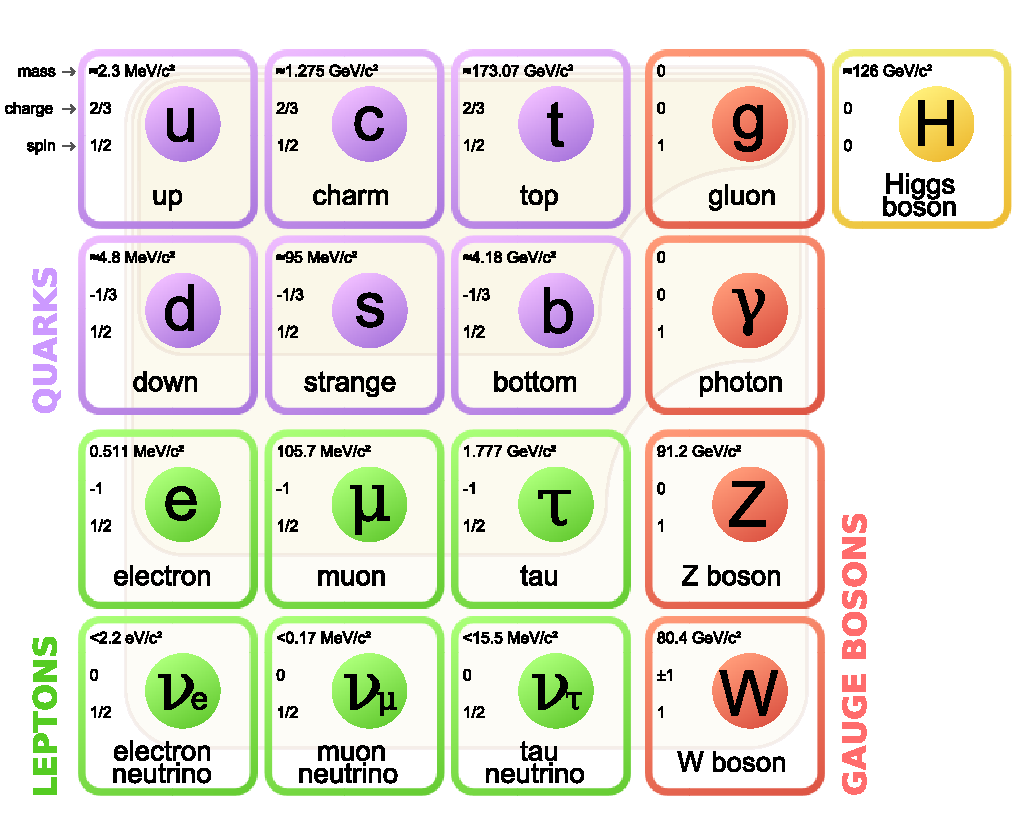
\includegraphics[width=0.7\textwidth]{figs/theory/standardmodel.pdf}
\caption{\label{fig:standardmodel} The particles in the standard model.}
\end{figure}

\begin{table}
\centering
\begin{tabular}{c|ccc}\hline\hline
field &$\mathrm{SU(3)}_{\mathrm{C}}$&$\mathrm{SU(2)}_{\mathrm{L}}$&$\mathrm{U(1)}_Y$ \\\hline
$q$ & $\mathbf{3}$ & $\mathbf{2}$ & $1/6$\\
$\overline u_\mathrm{R}$ & $\mathbf{\overline 3}$ & $\mathbf{1}$ & $-2/3$\\
$\overline d_\mathrm{R}$ & $\mathbf{\overline 3}$ & $\mathbf{1}$ & $1/3$\\
$\ell$ & $\mathbf{1}$ & $\mathbf{2}$ & $-1/2$\\
$\overline e_\mathrm{R}$ & $\mathbf{1}$ & $\mathbf{1}$ & $1$\\\hline
$h$ & $\mathbf{1}$ & $\mathbf{2}$ & $1/2$\\
\hline\hline
\end{tabular}
\caption{\label{tab:representations} Table summarizing the
    representations in which the matter fields transform under the standard
    model gauge group. $\mathbf{n}$ ($\mathbf{\overline n}$) is the
    fundamental (antifundamental) representation
    of $\mathrm{SU(n)}$. For the $\mathrm{U(1)}_Y$ factor, the
    representations are labeled by the weak hypercharge $Y$. The electric charge is given by $Q = T_{3L}+Y$. }
\end{table}


\section{Electroweak symmetry breaking}
\label{sec:ewsb}
A central feature of nonabelian gauge theories, or \emph{Yang-Mills theories}~\cite{Yang:1954ek}, is that the gauge bosons are
massless due to the fact that the gauge symmetry forbids explicit mass
terms in the Lagrangian. Thus Yang-Mills theory gives rise to massless
spin-$1$ particles. Concurrently, whenever a continuous
symmetry is \emph{spontaneously broken}\footnote{Spontaneous symmetry
  breaking means the equations of the dynamics are exactly symmetric,
  but they admit solutions that are not.}, \emph{Nambu-Goldstone
bosons}~\cite{Nambu:1960tm,Goldstone:1961eq} -- one for each generator of the broken symmetry -- appear in the spectrum of possible
excitations. These additional bosons are massless spin-$0$ particles. 

In the early 1960s, these massless bosons, both from nonabelian gauge
symmetry and spontaneous symmetry breaking, were seen as inconsistent with
nature since they were not observed. In 1962, Anderson realized a
mechanism for incorporating spontaneous symmetry breaking into nonrelativistic gauge
theories ``without any difficulties involving either zero-mass Yang-Mills gauge
bosons or zero-mass Goldstone bosons. These two
types of bosons seem capable of `canceling each other
out' and leaving finite mass bosons only''~\cite{Anderson:1963pc}. In
1964, this approach was extended to relativisitic gauge theories
through the introduction of a scalar field~\cite{PhysRevLett.13.321,HIGGS1964132,PhysRevLett.13.508,PhysRevLett.13.585,PhysRev.145.1156,PhysRev.155.1554}. In
the SM, the mechanism of electroweak symmetry breaking is a framework to keep the structure of gauge symmetry and
interactions at high energy, and still generate the observed masses
of the $\PW^{\pm}$ and $\PZ$ gauge
bosons~\cite{PhysRevLett.19.1264,GLASHOW1961579,Salam:1968rm}. 

The part of the SM Lagrangian that accomplishes this is: 
\begin{align}
\mathcal L_{\mathrm{Higgs}} &= (D_{\mu}\Phi)^{\dagger}(D^{\mu}\Phi) -
V(\Phi)~,& V(\Phi) &= -\mu^2\Phi^{\dagger}\Phi +
\lambda(\Phi^{\dagger}\Phi)^2~,
\label{eqn:Lhiggs}
\end{align}
where the field $\Phi$ is a complex, spin-$0$, self-interacting
$\mathrm{SU(2)}_{\mathrm{L}}$ doublet with weak hypercharge $Y=1/2$:
\begin{equation}
\Phi = \left(\begin{matrix} \phi^{+}\\\phi^0\end{matrix} \right)~.
\end{equation}
If $\mu^2>0$, then the potential will have a ``Mexican hat'' shape, illustrated in
\ref{fig:mexicanhat}, and the minimum of the potential will occur at a value of the field that is not $\mathrm{SU(2)}_{\mathrm{L}}\times\mathrm{U(1)}_Y$
invariant. Due to this, $\Phi$ acquires a nonzero vacuum
expectation value (\emph{vev}), corresponding to the minimum of the potential,
\begin{align}
\langle\Phi\rangle_0&\equiv \langle 0|\Phi|0\rangle =
\frac{1}{\sqrt{2}}U(x)\left(\begin{matrix} 0\\v\end{matrix} \right)~,&v &= \sqrt{\frac{\mu^2}{\lambda}}~,
\end{align}
where $U(x)$ is a unitary transformation that rotates the field
to the other degenerate solutions. Since the vev is still symmetric under a $\mathrm{U(1)}$ subgroup of the full
electroweak symmetry, we say the electroweak symmetry
$\mathrm{SU(2)}_{\mathrm{L}}\times\mathrm{U(1)}_Y$ is \emph{spontaneously
broken} to $\mathrm{U(1)}_{\mathrm{EM}}$. 

\begin{figure}
\centering
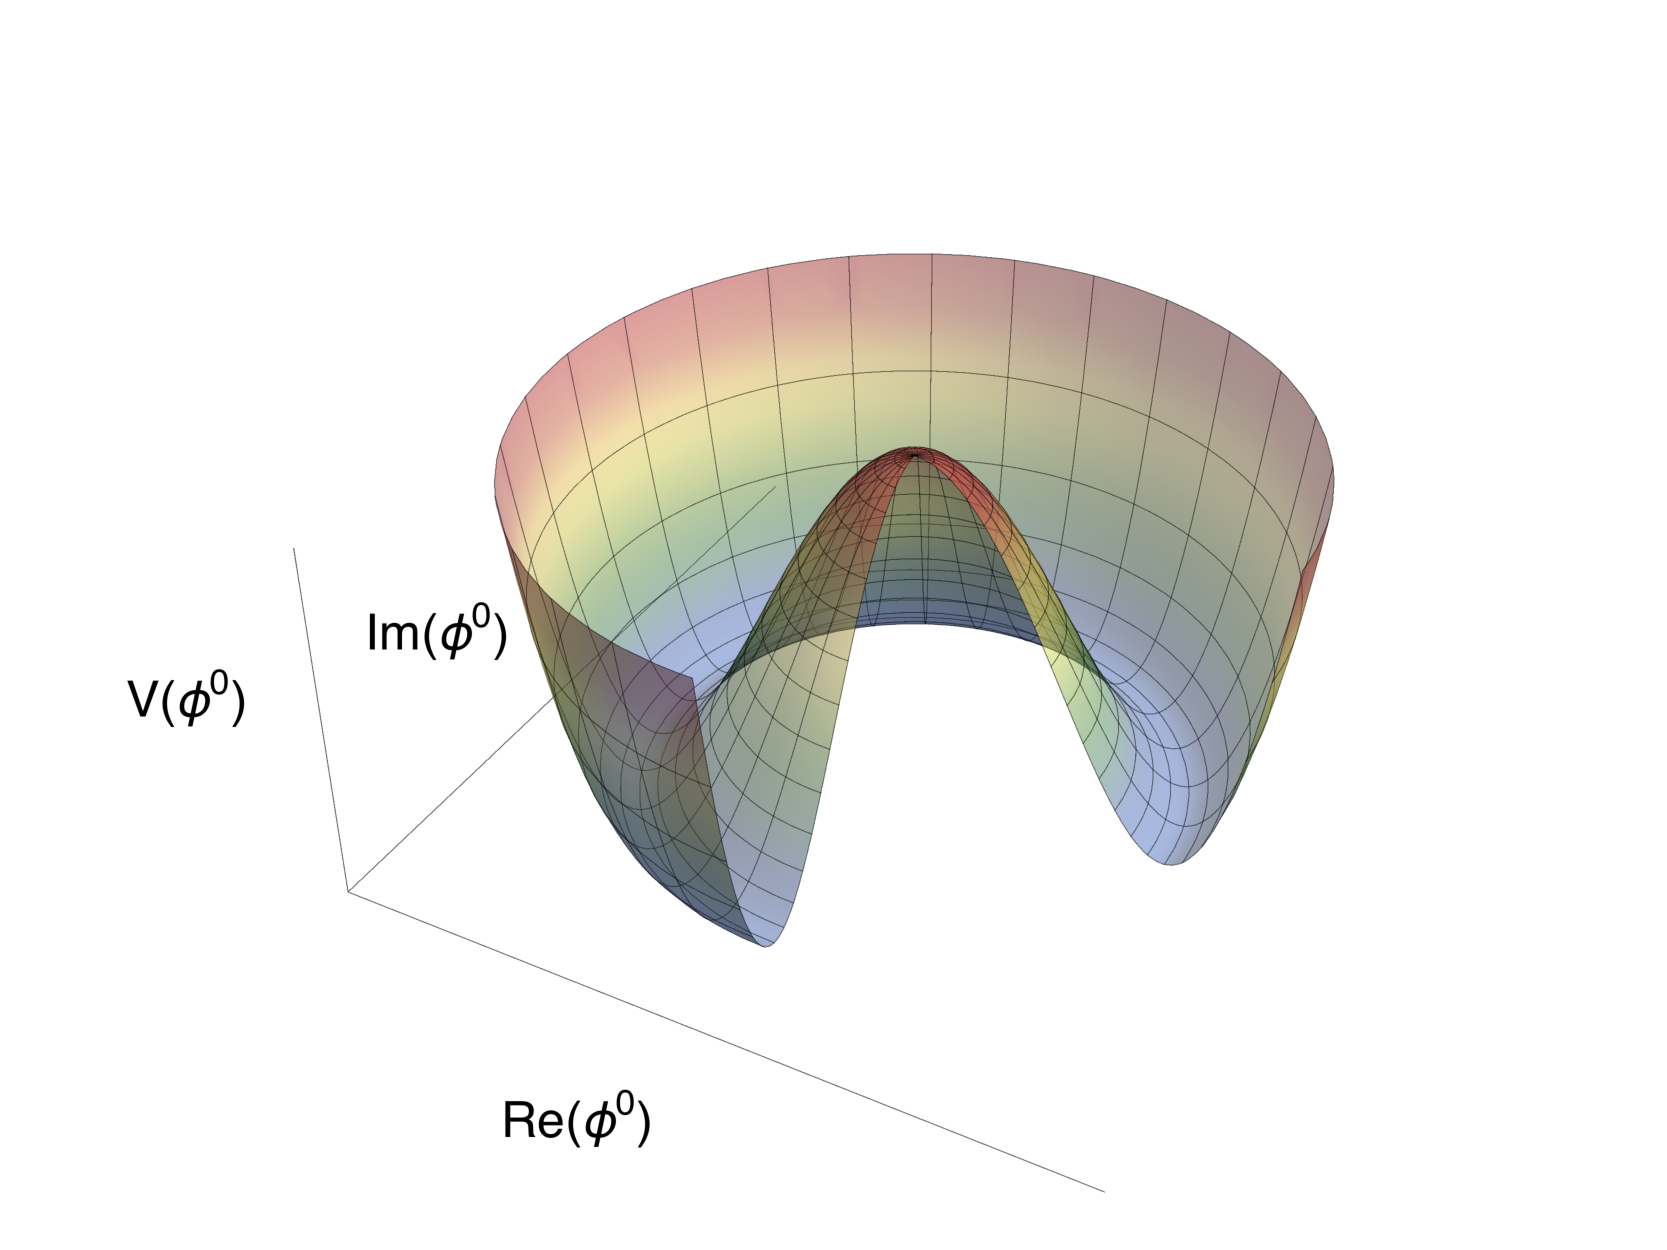
\includegraphics[width=0.7\textwidth]{figs/theory/MexicanHat.pdf}
\caption{\label{fig:mexicanhat} The shape of the ``Mexican hat''
  potential. The minimum of the potential occurs at
a field value that is not $0$~\cite{jmgd}.}
\end{figure}

This mechanism is responsible for generating the masses of the gauge
bosons in the SM, as can be seen by evaluating the 
covariant derivative in Eqn.~\ref{eqn:Lhiggs},
\begin{equation}
D_{\mu}\Phi = (\partial_{\mu} - i g_2 \frac{\sigma_a}{2}W^a_{\mu} -
ig_1\frac{1}{2}B_{\mu})\Phi ~,
\end{equation}
on the vacuum Higgs field. In this case, the kinetic term is:
\begin{align}
|D_{\mu}\Phi|^2 &= \frac{1}{2} \left|\left (\begin{matrix}\partial_{\mu}
    -\frac{i}{2}(g_2W_{\mu}^3 + g_1B_{\mu})&
    -\frac{ig_2}{2}(W_{\mu}^1-iW_{\mu}^2)\\ 
-\frac{ig_2}{2}(W_{\mu}^1+iW^2_{\mu})&\partial_{\mu}
    +\frac{i}{2}(g_2W_{\mu}^3 - g_1B_{\mu})
  \end{matrix}\right)
                                       \left(\begin{matrix}0\\v\end{matrix}\right)\right |^2 \nonumber\\
& = \frac{1}{8} \left ( g_2^2v^2|W_{\mu}^1+iW^2_{\mu}|^2 +
  v^2|g_2W^3_{\mu}-g_1B_{\mu}|^2 \right ) \nonumber\\
& = m_W^2W_{\mu}^+W^{-\mu} +
\frac{1}{2}m_Z^2Z_{\mu}Z^{\mu}~ + \frac{1}{2}m_{\gamma}^2A_{\mu}A^{\mu},
\end{align}
where we can identify three field combinations, $W_{\mu}^{\pm}$ and
$Z_{\mu}$, which have bilinear mass terms, and a fourth $A_{\mu}$,
which does not:
\begin{align}
W_{\mu}^{\pm} &= \frac{1}{\sqrt{2}}(W_{\mu}^1\mp iW^2_{\mu})~, &m_W &= \frac{1}{2}vg_2~,\\
Z_{\mu} &= \frac{g_2W_{\mu}^3 - g_1B_{\mu}}{\sqrt{g_1^2+g_2^2}}~,&m_Z &= \frac{1}{2}v\sqrt{g_1^2+g_1^2}~,\\
A_{\mu} &= \frac{g_2W_{\mu}^3 + g_1B_{\mu}}{\sqrt{g_1^2+g_2^2}}~,&m_{\gamma} &= 0.
\end{align}
The $\PW^{\pm}$ and $\PZ$ bosons have acquired mass, while the photon
$\Pgg$ remains massless.

An important consequence of this symmetry breaking mechanism is the
emergence of a physical spin-$0$ boson~\cite{HIGGS1964132,PhysRevLett.13.508}. If we expand the field around
its potential minimum
\begin{align}
\Phi(x)&=
\frac{1}{\sqrt{2}}U(x)\left(\begin{matrix} 0\\v+H(x)\end{matrix} \right)
\end{align}
and write out the terms associated to this field, we find
\begin{equation}
\mathcal L_{\mathrm{Higgs}} \supset \frac{1}{2}(\partial^{\mu}H)^2 -
\lambda v^2 H^2 - \lambda v H^3 - \frac{\lambda}{4}H^4~,
\end{equation}
which means this scalar boson, called the \emph{Higgs boson}, is self-interacting and has a mass squared of $m^2_\PH =
2\lambda v^2$ at tree-level.

\section{Fermion masses}
\label{sec:fermionmasses}
As proposed by Weinberg~\cite{PhysRevLett.19.1264}, fermions acquire
mass through interaction with the $\Phi$ field, which has a nonzero
vev. This is accomplished by adding Yukawa terms to the Lagrangian for
each generation,
\begin{equation}
\mathcal L_{\mathrm{Yukawa}} = - y_\Pe \overline\ell_\mathrm{L}\Phi e_\mathrm{R} -
y_\PQu\overline q_\mathrm{L}\Phi u_\mathrm{R}  - y_\PQd\overline q_\mathrm{L}\tilde\Phi d_\mathrm{R} + (\mathrm{h.c.})~,
\end{equation}
where the doublet $\tilde\Phi = i\sigma_2\Phi^{\ast}$ with hypercharge $Y=-1/2$ is
needed to generate masses for the down-type quarks. Then we can
identify the fermion masses as
\begin{align}
m_\Pe &= \frac{y_e v}{2}~,&m_\PQu &= \frac{y_\PQu
                                          v}{2}~,& m_\PQd &=
                                                          \frac{y_\PQd
                                                          v}{2}~.
\end{align}
%Neutrino masses can also be accommodated in the SM by adding similar
%terms. 
Besides giving masses to the fermions, the Yukawa terms have another important
consequence: they allow the fermions to affect the
observed mass of the Higgs boson through quantum corrections.

%\textbf{ Maurizio says: I would add a few lines about the tree-level Higgs mass. This connects to the next chapter}

\chapter{The hierarchy problem, naturalness, and supersymmetry}
\label{ch:naturalness}
\section{The hierarchy problem and naturalness in the standard model}
\label{sec:higgsnaturalness}

\textbf{Maria: Can you add after this section the beta functions if
  the self coupling and make a small subsection on the problem of the
  metastatibility of the vacuum. it involves again the looks, the top
  mass and the higgs mass (and as I guess) and it is an important
  point that Higgs is throwing us a curveball given the higgs mass and
  the top mass -- I think the traditional hierarchy and the problem of
  the metastability are the same problem just before and after the
  measurement of the higgs. Can point out that with SUSY included the
  metastability  problem is tossed in the garbage in the same way that
  SUSY is the answer to the hierarchy problem.}

The leading quantum correction to the Higgs mass is due to
the large Yukawa coupling of the top quark, which gives the
top quark its large mass. In an effective field theory approach, where
momenta of virtual particles are cut off at the scale
$\Lambda_{\mathrm{UV}}$, we can compute the top quark's contribution in the SM to leading order~\cite{susyprimer},
\begin{fmffile}{higgs1}
\begin{align}
m^2_\PH &= m^2_{\PH\mathrm{(bare)}} +\Delta(m^2_\PH) \\
\Delta(m^2_\PH) &= \quad\parbox{20mm}{
\begin{fmfgraph*}(20,20)
\fmfkeep{fermion}
\fmfleft{i} 
\fmfright{o} 
\fmf{dashes}{i,v1}
\fmf{dashes}{v2,o}
\fmf{plain,left,tension=.3,label=$t$}{v1,v2}
\fmf{plain,left,tension=.3}{v2,v1}
\fmfv{label=$\PH$,label.angle=90}{i}
\end{fmfgraph*}} \quad + \quad\cdots\\
&= -\frac{3|y_\PQt|^2}{8\pi^2}\Lambda_{\mathrm{UV}}^2 + \cdots~,
\label{eqn:toploop}
\end{align}
\end{fmffile}
The quadratic dependence in Eqn.~\ref{eqn:toploop} on
$\Lambda_{\mathrm{UV}}$, usually taken to be the Planck scale $10^{19}
\GeV$, means the Higgs mass is sensitive to new physics in the
ultraviolet. Taken literally, this sensitivity implies an enormous fine tuning of
$m^2_{\PH\mathrm{(bare)}}$ to achieve almost perfect
cancellation\footnote{to $1$ part in $10^{34}$} with
$\Delta(m^2_\PH)$ in order to explain how $m_\PH$
is measured to be so small at $125.09\pm0.24 \GeV$~\cite{Aad:2015zhl}. The conundrum of how a light fundamental
scalar particle can exist in the presence of (presumably) new physics
in the ultraviolet is called the \emph{hierarchy problem} or the \emph{naturalness problem} and is one
of the key motivations for new physics at the \TeV scale, especially \emph{supersymmetry}.

\section{Renormalization group running in the standard model}
\label{sec:rgesm}
In the renormalization group (RG) approach to quantum field theory,
the Lagrangian parameters may be thought of as
``running'' parameters that depend on the energy scale $\mu$ of a
given physical process. The beta function $\beta(g)$ encodes the dependence of a coupling $g$
on $\mu$,
\begin{equation}
\beta(g) = \frac{\rd g}{\rd \log\mu}~.
\end{equation}
By integrating the beta function, we obtain a
relationship between the couplings evaluated at different energy scales. The beta
functions for the gauge couplings in the SM may be computed by considering loop diagrams up to a
certain order. The one-loop beta functions for  $g_1 = \sqrt{5/3}g^{\prime}$, $g_2 =g$,
and $g_3 = g_\mathrm{s}$ are
\begin{align}
\frac{\rd g_1}{\rd\log\mu} &= \frac{g_1^3}{20\pi^2} \left (\sum_{\textrm{Weyl ferm.}}\frac{1}{2}Y^2+\sum_{\mathbb C\textrm{ scalars}}\frac{1}{4}Y^2\right)\\
&=\frac{g_1^3}{20\pi^2} \left( \frac{41}{8} \right)~,\\
\frac{\rd g_2}{\rd\log\mu} &= \frac{g_2^3}{16\pi^2} \left (-\frac{11}{3} \times 2 + \frac{2}{3}\sum_{\textrm{Weyl ferm.}\in\mathbf{2}}\frac{1}{2}+\frac{2}{3}\sum_{\mathbb C \textrm{ scalars}\in\mathbf 2}\frac{1}{4}\right)\\
&= \frac{g_2^3}{16\pi^2}\left( -\frac{19}{6} \right)~,\\
\frac{\rd g_3}{\rd\log\mu} &=\frac{g_3^3}{16\pi^2} \left (-\frac{11}{3} \times 3 + \frac{2}{3}\sum_{\textrm{Weyl ferm.}\in\mathbf{3}}\frac{1}{2} \right)\\
&= \frac{g_3^3}{16\pi^2}\left( -7\right)~,
\end{align}
where $g_\mathrm{s}$, $g$, and $g^{\prime}$ are the gauge couplings
for the gauge groups $\mathrm{SU(3)}_{\mathrm{C}}$,
$\times\mathrm{SU(2)}_{\mathrm{L}}$, and $\times\mathrm{U(1)}_Y$,
respectively. The running of these couplings, extrapolated all the way up to
the Planck scale (assuming there is no new physics) is shown in
Fig.~\ref{smphase} using with the three-loop RG equations and
including the two-loop threshold corrections at the weak
scale~\cite{Buttazzo:2013uya}. Given the particle content of the SM
and assuming no additional particles, the gauge couplings do
not appear to unify near the mass scale of $10^{16}\GeV$, an essential feature
of grand unification theories (GUT)~\cite{Georgi:1974sy,susyprimer}.

\subsection{Vacuum instability}
\label{sec:vacuuminstability}
The one-loop beta functions for the top-quark Yukawa
coupling $y_\PQt$ and the Higgs quartic coupling $\lambda$ in the SM
may be computed similarly:
\begin{align}
16\pi^2\frac{\rd y_\PQt}{\rd\log\mu} &= -\frac{17}{20}g_1^2y_\PQt - \frac{9}{4}g_2^2y_\PQt  - 8g_3^2y_\PQt + \frac{9}{2}y_\PQt^3~,\\
16\pi^2\frac{\rd \lambda}{\rd\log\mu} &= -\frac{9}{5}g_1^2\lambda - 9g_2^2\lambda + \frac{27}{100}g_1^4 + \frac{9}{10}g_2^2g_1^2 + \frac{9}{4}g_2^4 + 12\lambda^2  +12\lambda y_\PQt^2 - 12y_\PQt^4~.\\
\end{align}
The running of the $\lambda$ is of particular interest because if it
runs to $\lambda<0$, in principle 
From these two Lagrangian parameters, we can visualize the SM phase
diagram in ($m_\PH$, $m_\PQt$), divided into regions of absolute
stability ($\lambda>0$ for all $\mu$), metastability ($\lambda<0$ for
large $\mu$ near the Planck scale), and instability ($\lambda<0$ for
small $\mu$ near the weak scale). Ref.~\cite{Buttazzo:2013uya}
computes with three-loop RG equations and two-loop threshold
corrections at the weak scale as seen in
Fig.~\ref{fig:smphase}. Curiously, if the SM is valid up to the Planck
scale, the SM vacuum appears to be metastable and very close to the
boundary between metastability and absolute stability~\cite{Buttazzo:2013uya}.

\begin{figure}
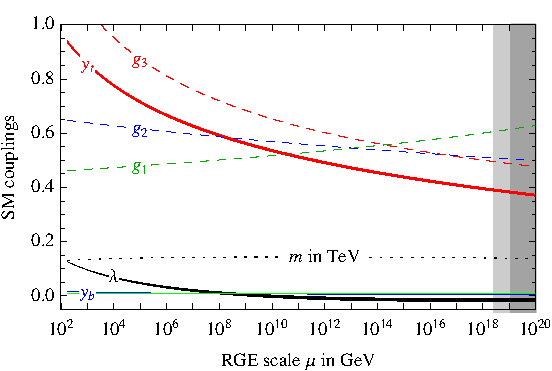
\includegraphics[width=0.49\textwidth]{figs/theory/SMRGE.pdf}\\
%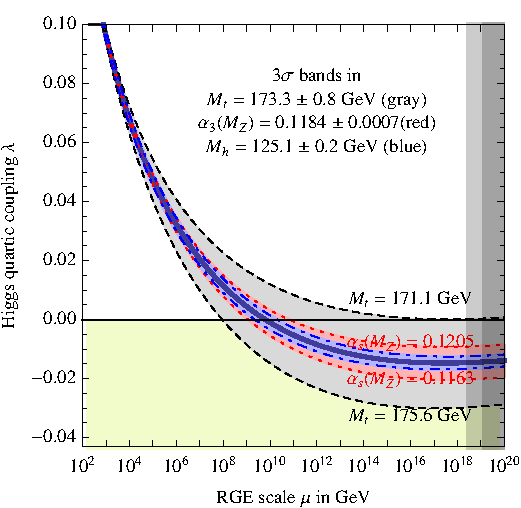
\includegraphics[width=0.49\textwidth]{figs/theory/lambda.pdf}\\
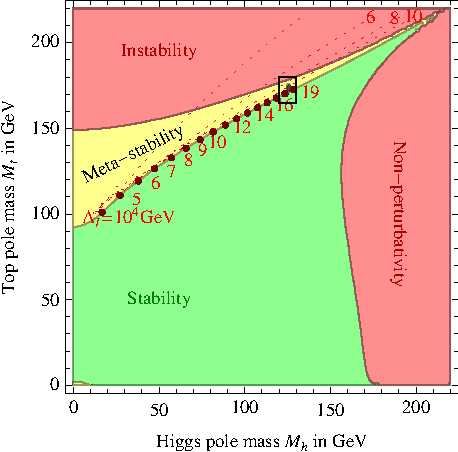
\includegraphics[width=0.49\textwidth]{figs/theory/SMht.pdf}\\
%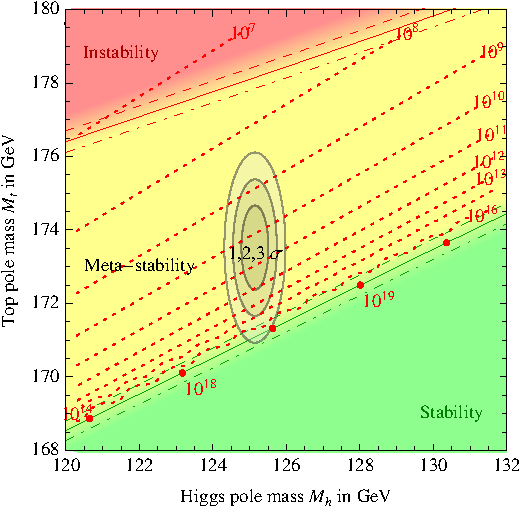
\includegraphics[width=0.49\textwidth]{figs/theory/deadoraliveG2014}\\
\caption{Renormalization of the SM gauge couplings $g_1 =
\sqrt{5/3}g^{\prime}$, $g_2$, $g_3$, of the top, bottom and $\tau$
couplings ($y_\PQt$, $y_\PQb$, $y_\tau$), of the Higgs quartic
coupling $\lambda$, and of the Higgs mass parameter $m_\PH$ (left) and SM phase diagram in terms of Higgs and top pole masses (right).
%All parameters are defined in the $\overline{\mathrm{MS}}$ scheme. The
%two-loop thresholds at the weak scale and three-loop RG equations. The thickness indicates the ±1σ uncertainties in Mt
%, Mh, α3. 
The plane is divided into regions of absolute stability, metastability, instability of the SM vacuum, and nonperturbativity
of the Higgs quartic coupling. The top Yukawa coupling becomes non-perturbative
for $m_{\PQt} > 230 \GeV$. The dotted contour-lines show the instability scale
$\Lambda_\mathrm{I}$ assuming $\alpha_3(m_\PZ) = 0.1184$~\cite{Buttazzo:2013uya}.\label{fig:smphase}}
%Zoom in the region of the preferred experimental range of $m_\PH$ and $m_\PQt$
%(the grey areas denote the allowed region at $1$, $2$, and $3\sigma$). The three boundary lines correspond
%to $1-\sigma$ variations of $\alpha_3(m_{\PZ}) = 0.1184\pm 0.0007$, and the grading of the colours indicates the size
%of the theoretical error~\cite{Buttazzo:2013uya}.}
\end{figure}

\section{Supersymmetry}
\label{sec:susy}
Supersymmetry (SUSY) is a proposed symmetry of spacetime that 
introduces a bosonic (fermionic) partner for every fermion
(boson)~\cite{Wess,Golfand,Volkov,Chamseddine,Kane,Fayet,Barbieri,Hall,Ramond}. For
many years, such a symmetry was thought to be impossible since in 1967,
Coleman and Mandula~\cite{PhysRev.159.1251} published their no-go theorem that says
internal symmetries, those that act on internal degrees of
freedom (like spin) cannot be combined with spacetime symmetries in a
nontrivial way. SUSY evades this theorem because it is based
on a \emph{super Lie algebra}, which may include fermionic symmetries
and anticommutation relations as well as the usual bosonic symmetries
and commutation relations.

Supersymmetric extensions of the SM are compelling mainly because they 
\begin{enumerate}[(a)]
\item yield a solution to the hierarchy problem, alleviating
the fine-tuning of fundamental
parameters~\cite{Witten:1981nf,Dimopoulos:1981zb,Dine:1981za,Dimopoulos:1981au,Sakai:1981gr,Kaul:1981hi},
explained further in Sec.~\ref{sec:susynaturalness}.
\item exhibit gauge coupling
  unification~\cite{Dimopoulos:1981yj,Marciano:1981un,Einhorn:1981sx,Ibanez:1981yh,Amaldi:1991cn,Langacker:1995fk}, and
\item provide a weakly interacting particle candidate for dark matter~\cite{Ellis:1983ew,Jungman:1995df}.
\end{enumerate}

SUSY can be thought of as an extension of the usual group of spacetime
symmetries, known as the Poincar\'{e} group. This group has
generators related to translation symmetry, $P_m$, and Lorentz
symmetry, $M_{mn} = -M_{nm}$, which form a Lie algebra:
\begin{align}
~[P_m,P_n] &= 0 \nonumber\\
~[P_m,M_{np}] &= i(\eta_{mn}P_p-\eta_{mp}P_n) \nonumber\\
~[M_{mm},M_{pq}] &= i(\eta_{mp}M_{np} - \eta_{np}M_{mq} +
                   \eta_{nq}M_{mp} - \eta_{mq}M_{np} )~.
\label{eqn:poincare}
\end{align}

As shown by Coleman and Mandula~\cite{PhysRev.159.1251}, the only way
to extend this symmetry with a new internal symmetry group $G$ with bosonic
generators $B_r$ and Lie algebra,
\begin{equation}
~[B_r,B_s] = f_{rs}{}^tB_t~,
\end{equation}
with structure functions $f_{rs}{}^t$, is if the extended symmetry
group is simply the direct product $($Poincar\'{e}$)\times G$ with a
trivial Lie algebra,
\begin{equation}
~[B_r,P_m] = [B_r,M_{mn}] = 0~.
\end{equation}

However, SUSY exploits a loophole in the Coleman-Mandula theorem,
which only considers bosonic symmetry generators, by incorporating
fermionic symmetry generators $Q$ that generate SUSY transformations,
\begin{equation}
Q|\mathrm{boson}\rangle = |\mathrm{fermion}\rangle, ~~~~
Q|\mathrm{fermion}\rangle = |\mathrm{boson}\rangle~.
\end{equation}
Supersymmetries can be combined with the
spacetime symmetries in a way that mixes the two symmetries, as
exemplified by the super Lie algebra for $\mathcal N=1$
SUSY,
\begin{align}
~\{ Q_{\alpha},\overline Q_{\dot{\beta}}\} &= 2\sigma^m_{\alpha\dot\beta} P_m \nonumber\\
~\{ Q_{\alpha},Q_{\beta}\} &= \{ \overline Q_{\dot\alpha},\overline Q_{\dot\beta}\} = 0\nonumber\\
~[ P_m, Q_{\alpha}] &= [P_m,\overline Q_{\dot\alpha}] = 0~.
\label{eqn:n1susy}
\end{align}
In other words, two SUSY generators can combine to generate a spacetime translation.

The most economical supersymmetric extension of the standard model is the
Minimal Supersymmetric Standard Model (MSSM). For supersymmetric
theories, the Lagrangian can be written in terms of vector superfields
$V(x,\theta,\overline\theta)$ and chiral superfields $\Phi_l(x,\theta,\overline\theta)$ that are functions of
\emph{superspace}, an extension of spacetime that includes
anticommuting Grassmanian variables $\theta$ and
$\overline\theta$. Tab~\ref{tab:susyreps} shows the particles of the
MSSM, described by chiral superfields $Q_i, U_i^\mathrm{c}, L_i, E_i^\mathrm{c}, H_\PQu,
H_\PQd$, and the representations in which they transform under the MSSM gauge group.
\begin{table}
\centering
\begin{tabular}{c|ccc}\hline\hline
&$\mathrm{SU(3)}_{\mathrm{C}}$&$\mathrm{SU(2)}_{\mathrm{L}}$&$\mathrm{U(1)}_Y$ \\\hline
$Q$ & $\mathbf{3}$ & $\mathbf{2}$ & $1/6$\\
$U^\mathrm{c}$ & $\mathbf{\overline 3}$ & $\mathbf{1}$ & $-2/3$\\
$D^\mathrm{c}$ & $\mathbf{\overline 3}$ & $\mathbf{1}$ & $1/3$\\
$L$ & $\mathbf{1}$ & $\mathbf{2}$ & $-1/2$\\
$E^\mathrm{c}$ & $\mathbf{1}$ & $\mathbf{1}$ & $1$\\\hline
$H_\PQu$ & $\mathbf{1}$ & $\mathbf{2}$ & $1/2$\\
$H_\PQd$ & $\mathbf{1}$ & $\mathbf{2}$ & $-1/2$\\
\hline\hline
\end{tabular}
\caption{\label{tab:susyreps} Table summarizing the
    representations in which the chiral superfields transform under
    the MSSM gauge group. See Tab.~\ref{tab:representations} for a
    description of the columns.}
\end{table} 

The MSSM Lagrangian can be split into three terms, the K\"{a}hler potential $K(\Phi_l,\Phi_l^{\dagger},V)$,
which describes the kinetic and gauge-covariant terms, a superpotential $W(\Phi_l)$, which
describes the mass and interaction terms, and a gauge kinetic term $G(V)$,
\begin{align}
\mathcal L_{\mathrm{MSSM}} &= \int \mathrm{d}^4\theta
K(\Phi_l,\Phi_l^{\dagger},V) + \left (\int
 \mathrm{d}^2\theta W(\Phi_l) + \mathrm{h.c.} \right) + \left (\int
\mathrm{d}^2\theta G(V) +
\mathrm{h.c.}\right )\nonumber\\
&= \int \mathrm{d}^4\theta
\sum_{V}
\Phi_{l}^{\dagger}e^{gV}\Phi_{l} + \left (\int
 \mathrm{d}^2\theta W(\Phi_l) + \mathrm{h.c.} \right) + \left (\int
\mathrm{d}^2\theta \frac{1}{4}\mathcal W^{\alpha}\mathcal W_{\alpha} +
\mathrm{h.c.}\right )~,
\label{eqn:mssmlag}
\end{align}
where $\mathcal W_{\alpha}$ is the vector superfield strength\footnote{The vector superfield strength is $\mathcal W_{\alpha} =
  -\frac{1}{4} \overline{\mathcal{D}}^2(e^{-V}\mathcal{D}_{\alpha}
  e^{V})$.} and the index $l$ runs over all the matter superfields
$\Phi_l = Q_i, U_i^\mathrm{c}, L_i, E_i^\mathrm{c}, H_\PQu, H_\PQd$. The superpotential can be
split into two components based on $R$-parity, a discrete $Z_2$
symmetry often assumed in SUSY model building, defined for each
particle as 
\begin{equation}
P_R = (-1)^{3(\mathrm{B}-\mathrm{L})+2s}~,
\end{equation}
where $\mathrm{B}$ is the baryon number, $\mathrm{L}$ is the lepton number, and $s$ is the spin
of the particle. With this assignment, all SM particles have even
$R$-parity ($P_R=+1$), while the superpartners have odd $R$-parity
($P_R=-1$). The $R$-parity conserving terms in the superpotential are
\begin{equation}
W_{\mathrm{RPC}} = - U^\mathrm{c}\mathbf{y_\PQu} Q H_\PQu + D^\mathrm{c}\mathbf{y_\PQd}QH_\PQd  +
E^\mathrm{c}\mathbf{y_e} L H_\PQd +
\mu H_\PQu H_\PQd~,
\label{eqn:Wrpc}
\end{equation}
and the $R$-parity violating terms are
\begin{equation}
W_{\mathrm{RPV}} =\frac{1}{2}\lambda^{ijk}L_iL_jE_k^\mathrm{c} +
\lambda^{\prime ijk} L_iQ_jD_k^\mathrm{c} + \mu^{\prime i}H_\PQu L_i +
\frac{1}{2}\lambda^{\prime\prime ijk}U_i^\mathrm{c}D_j^\mathrm{c}D_k^\mathrm{c}~.
\label{eqn:Wrpv}
\end{equation}

If $R$-parity is conserved, there are three important phenomenological consequences:
\begin{itemize}
\item The lightest superparter, called the ``lightest
  supersymmetric particle'' or LSP, must be stable. 
\item Each superpartner other than the LSP must eventually decay into a
  state that contains an odd number of LSPs (usually just one).
\item In collider experiments, superpartners can only be produced in even numbers (usually two).
\end{itemize}
In particular, at a proton-proton collider like the LHC (described in
Ch.~\ref{ch:lhc}), the SUSY processes with the largest cross
sections are the pair production of gluinos and squarks through
gluon-gluon and gluon-quark fusion, which are among the reactions of QCD-level
strength~\cite{susyprimer}:
\begin{align}
\Pg\Pg&\to \sGlu\sGlu, \PSq_i\overline{\PSq}_j~,\label{eqn:gg}\\
\Pg\Pq&\to \sGlu\PSq_i~,\\
\Pq\Paq&\to \sGlu\sGlu,\PSq_i\overline{\PSq}_j~,\\
\Pq\Pq&\to \PSq_i\PSq_j~.
\end{align}
Some of the diagrams corresponding to the gluon-gluon fusion reactions in
Eqn.~\ref{eqn:gg} are depicted in
Fig.~\ref{fig:gg}~\cite{susyprimer}. Assuming all SUSY particles other than those being pair-produced
are decoupled from the theory (as is done in the simplified model
approach, see Sec.~\ref{sec:sms}~\cite{ArkaniHamed:2007fw,Alwall:2008ag,Alwall:2008va,Alves:2011sq,Alves:2011wf,Graesser:2012qy}), the SUSY pair-production cross sections for
each SUSY particle may be computed at next-to-leading-order (NLO) plus
next-to-leading-logarithm (NLL)
accuracy~\cite{NLONLL1,NLONLL2,NLONLL3,NLONLL4,NLONLL5,NLONLLerr,Borschensky:2014cia}. For
the $\sqrt{s}=8\TeV$ and $13\TeV$ LHC, these SUSY production cross sections are plotted as a function of the
superpartner mass in Fig.~\ref{fig:xsecsusy}. Due to the hierarchy of SUSY
cross sections, there is a corresponding hierarchy in terms of
discovery potential at the LHC, with the largest mass reach for
gluinos then squarks then top and bottom squarks then electroweak SUSY
partners (see Sec.\ref{sec:ewksusy}) then, finally, sleptons.

\begin{figure}[h!]
\centering
  \unitlength=0.005\textwidth
  \vspace{\baselineskip}
\setkeys{Gin}{width=\ginnatwidth,totalheight=\ginnatheight}
\begin{fmffile}{gg}
\begin{fmfgraph*}(60,30)
        \fmfset{arrow_len}{cm}\fmfset{arrow_ang}{0}
         \fmfleftn{i}{2}
         \fmfrightn{o}{2}
             \fmf{gluon}{v1,i1}
             \fmf{gluon}{v1,i2}    
             \fmf{gluon, lab=$\mathrm{g}$,label.side=left}{v1,v2}                    
           \fmf{gluon}{v2,o2} %upper vertex
           \fmf{gluon}{v2,o1} %lower vertex 
           \fmffreeze
           \fmflabel{$\mathrm{g}$}{i1}
         \fmflabel{$\mathrm{g}$}{i2}
           \fmflabel{\sGlu}{o2}
         \fmflabel{\sGlu}{o1}
           \fmf{fermion}{v2,o2}
          \fmf{fermion}{v2,o1}
      \fmfdot{v1,v2}
  \end{fmfgraph*}
\hfill 
\begin{fmfgraph*}(60,30)
        \fmfset{arrow_len}{cm}\fmfset{arrow_ang}{0}
         \fmfleftn{i}{2}
         \fmfrightn{o}{2}
         \fmfbottom{i1,d1,o1}
         \fmftop{i2,d2,o2}
             \fmf{gluon}{i1,v1}
             \fmf{gluon}{i2,v2}    
             \fmf{gluon, lab=\sGlu,label.side=left,tension=0}{v1,v2}                    
           \fmf{gluon}{v1,o1} %lower vertex
           \fmf{gluon}{v2,o2} %upper vertex 
           \fmffreeze
           \fmflabel{$\mathrm{g}$}{i1}
         \fmflabel{$\mathrm{g}$}{i2}
           \fmflabel{\sGlu}{o2}
         \fmflabel{\sGlu}{o1}
           \fmf{fermion}{v1,o1}
          \fmf{fermion}{v2,o2}
          \fmf{fermion}{v1,v2}
      \fmfdot{v1,v2}
  \end{fmfgraph*}\\
  \vspace{3\baselineskip}
\begin{fmfgraph*}(60,30)
        \fmfset{arrow_len}{cm}\fmfset{arrow_ang}{0}
         \fmfleftn{i}{2}
         \fmfrightn{o}{2}
             \fmf{gluon}{v1,i1}
             \fmf{gluon}{v1,i2}    
             \fmf{gluon, lab=$\mathrm{g}$,label.side=left}{v1,v2}                    
           \fmf{dashes}{v2,o2} %upper vertex
           \fmf{dashes}{v2,o1} %lower vertex 
           \fmffreeze
           \fmflabel{$\mathrm{g}$}{i1}
         \fmflabel{$\mathrm{g}$}{i2}
           \fmflabel{$\PSq$}{o2}
         \fmflabel{$\overline\PSq$}{o1}
      \fmfdot{v1,v2}
  \end{fmfgraph*}\hfill
\begin{fmfgraph*}(60,30)
        \fmfset{arrow_len}{cm}\fmfset{arrow_ang}{0}
         \fmfleftn{i}{2}
         \fmfrightn{o}{2}
         \fmfbottom{i1,d1,o1}
         \fmftop{i2,d2,o2}
             \fmf{gluon}{i1,v1}
             \fmf{gluon}{i2,v2}    
             \fmf{dashes, lab=$\PSq$,label.side=left,tension=0}{v1,v2}                    
           \fmf{dashes}{v1,o1} %lower vertex
           \fmf{dashes}{v2,o2} %upper vertex 
           \fmffreeze
           \fmflabel{$\mathrm{g}$}{i1}
         \fmflabel{$\mathrm{g}$}{i2}
           \fmflabel{$\PSq$}{o2}
         \fmflabel{$\overline\PSq$}{o1}
      \fmfdot{v1,v2}
  \end{fmfgraph*}\hfill
\begin{fmfgraph*}(45,30)
        \fmfset{arrow_len}{cm}\fmfset{arrow_ang}{0}
         \fmfleftn{i}{2}
         \fmfrightn{o}{2}
             \fmf{gluon}{v1,i1}
             \fmf{gluon}{v1,i2}                
           \fmf{dashes}{v1,o2} %upper vertex
           \fmf{dashes}{v1,o1} %lower vertex 
           \fmffreeze
           \fmflabel{$\mathrm{g}$}{i1}
         \fmflabel{$\mathrm{g}$}{i2}
           \fmflabel{$\PSq$}{o2}
         \fmflabel{$\overline\PSq$}{o1}
      \fmfdot{v1}
  \end{fmfgraph*}
\end{fmffile}\setkeys{Gin}{width=\linewidth,totalheight=\textheight,keepaspectratio}
  \vspace{\baselineskip}
\caption{Example diagrams for the production of gluinos and squarks from gluon-gluon fusion~\cite{susyprimer}. \label{fig:gg}}
\end{figure}

\begin{figure}
\centering
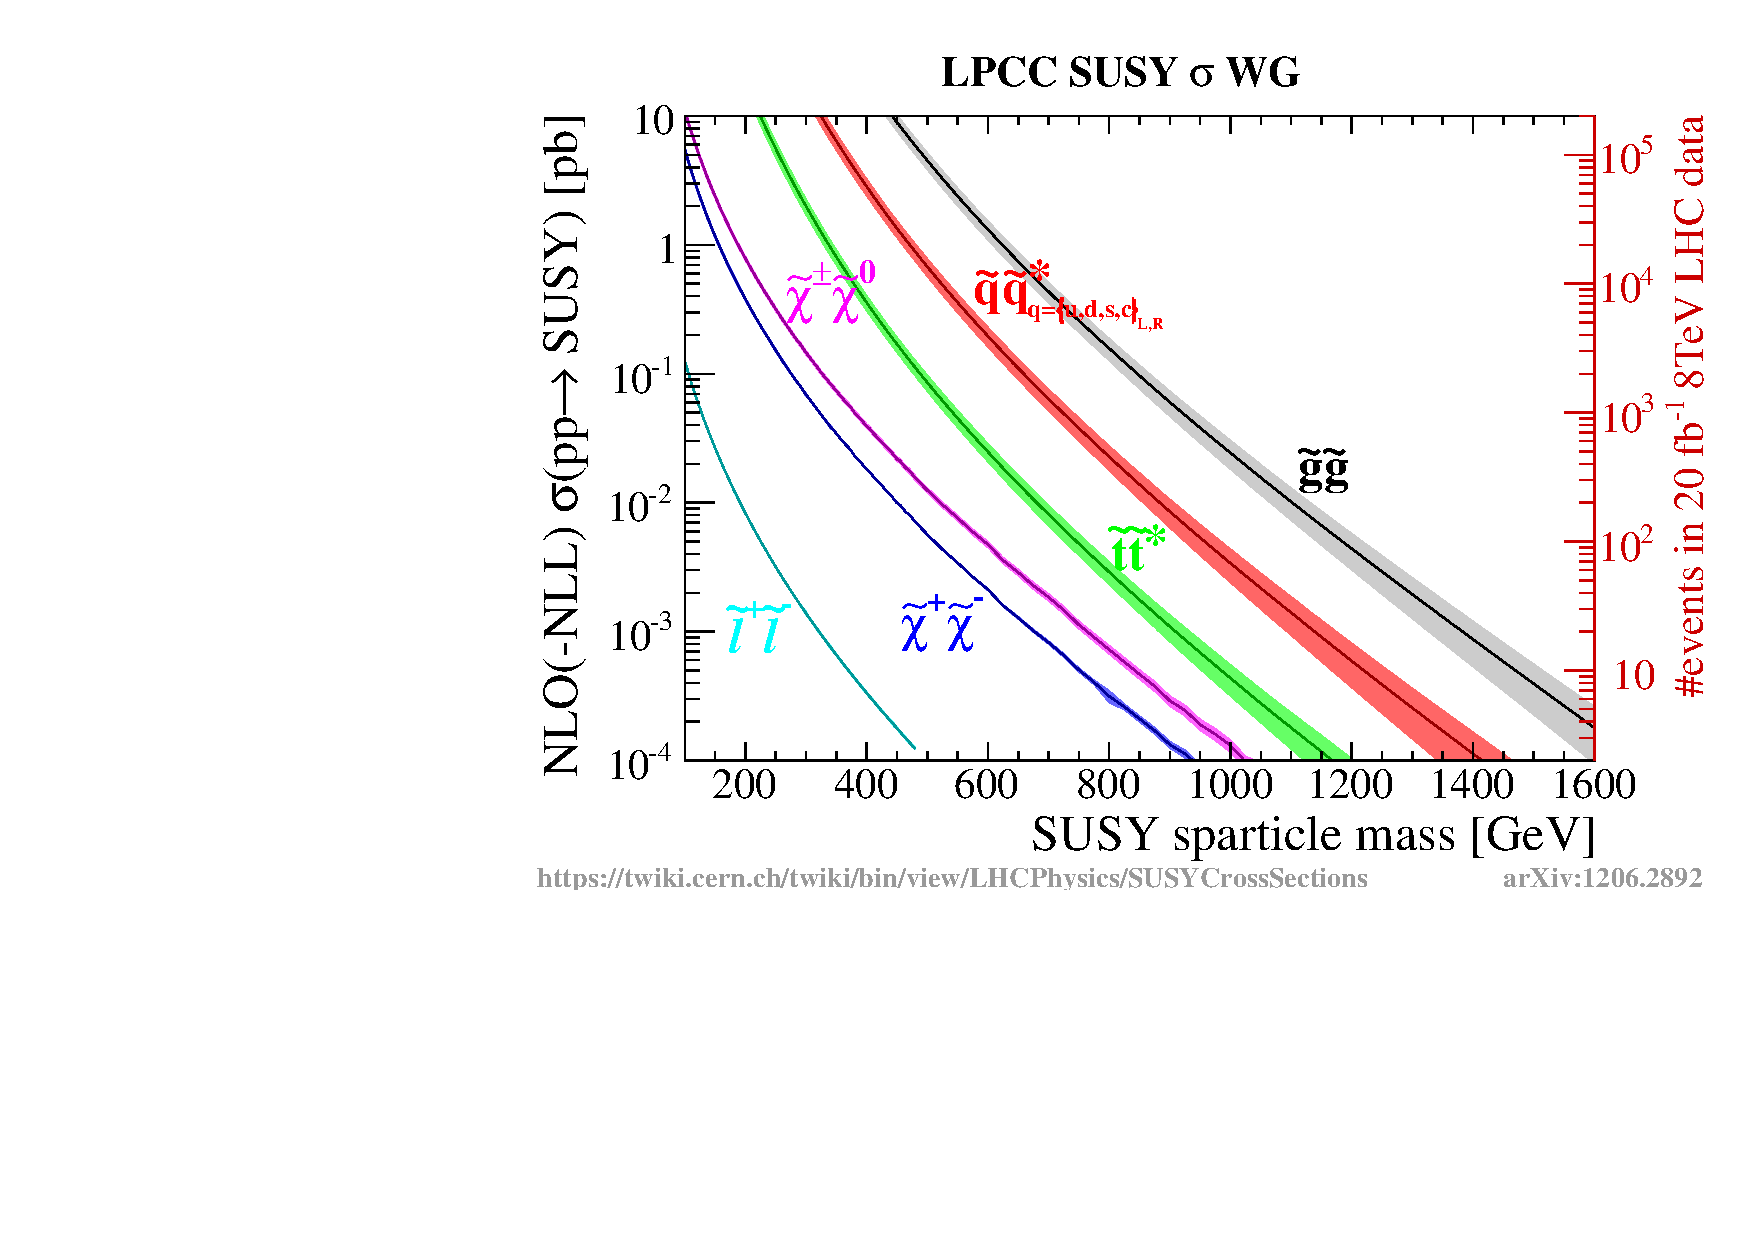
\includegraphics[width=0.9\textwidth]{figs/theory/xsections_strong.pdf}\\
%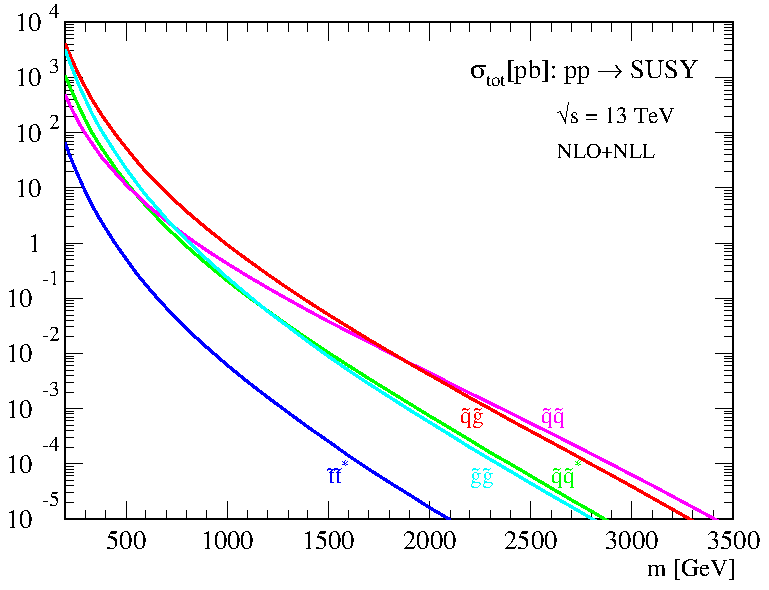
\includegraphics[width=0.7\textwidth]{figs/theory/nlonll_lhc13_col.pdf}
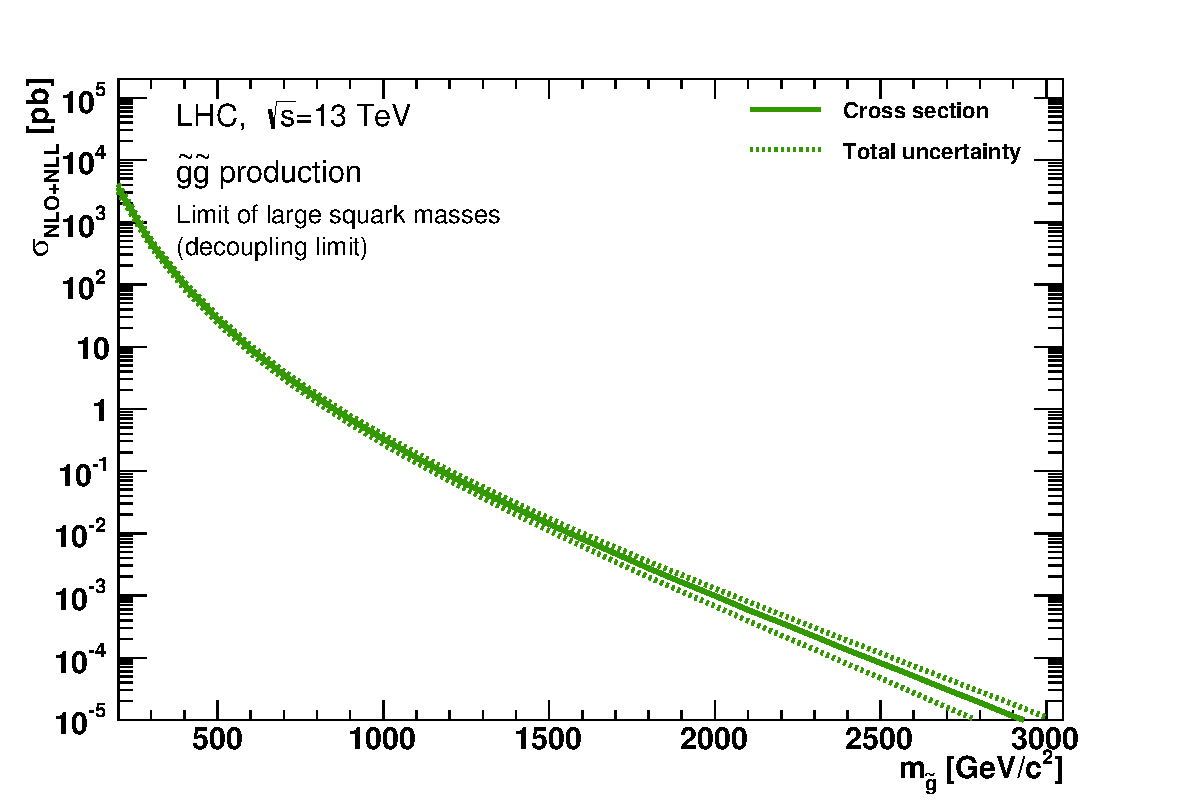
\includegraphics[width=0.3\textwidth]{figs/theory/xsec_gg_200_3050.pdf}
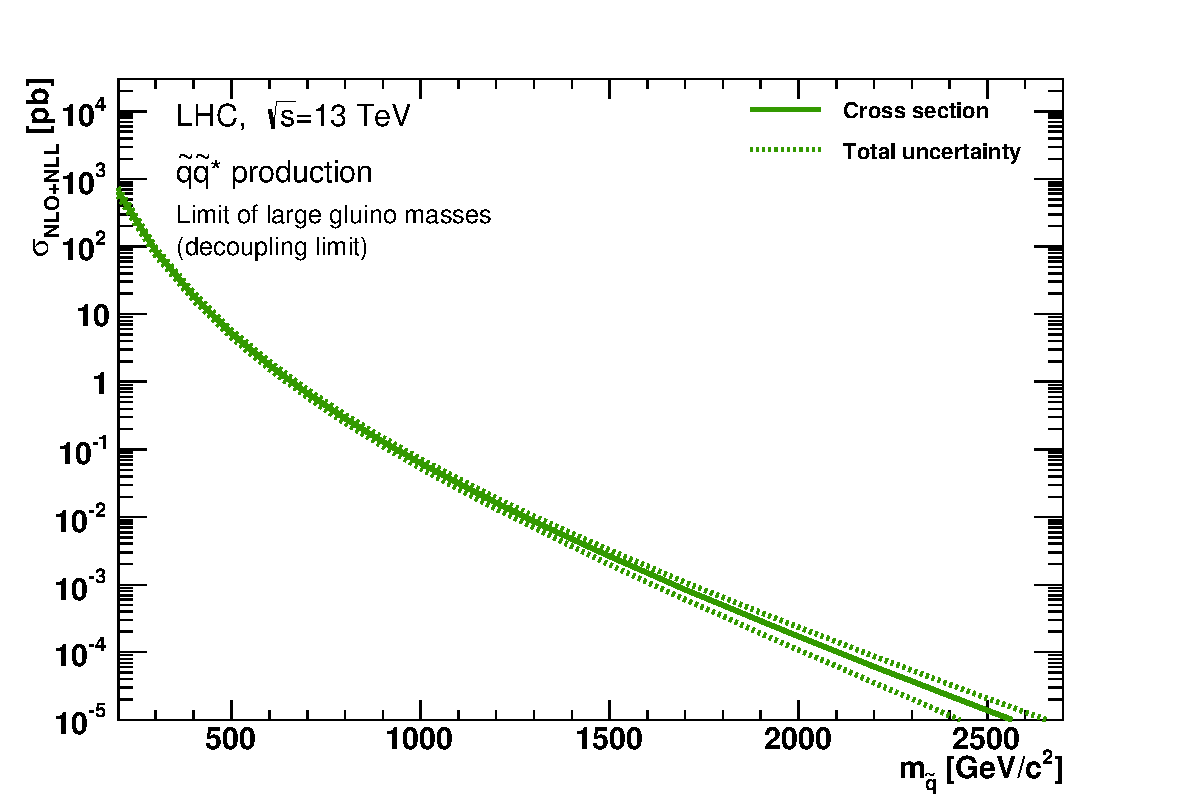
\includegraphics[width=0.3\textwidth]{figs/theory/xs_squark_200_2700.pdf}
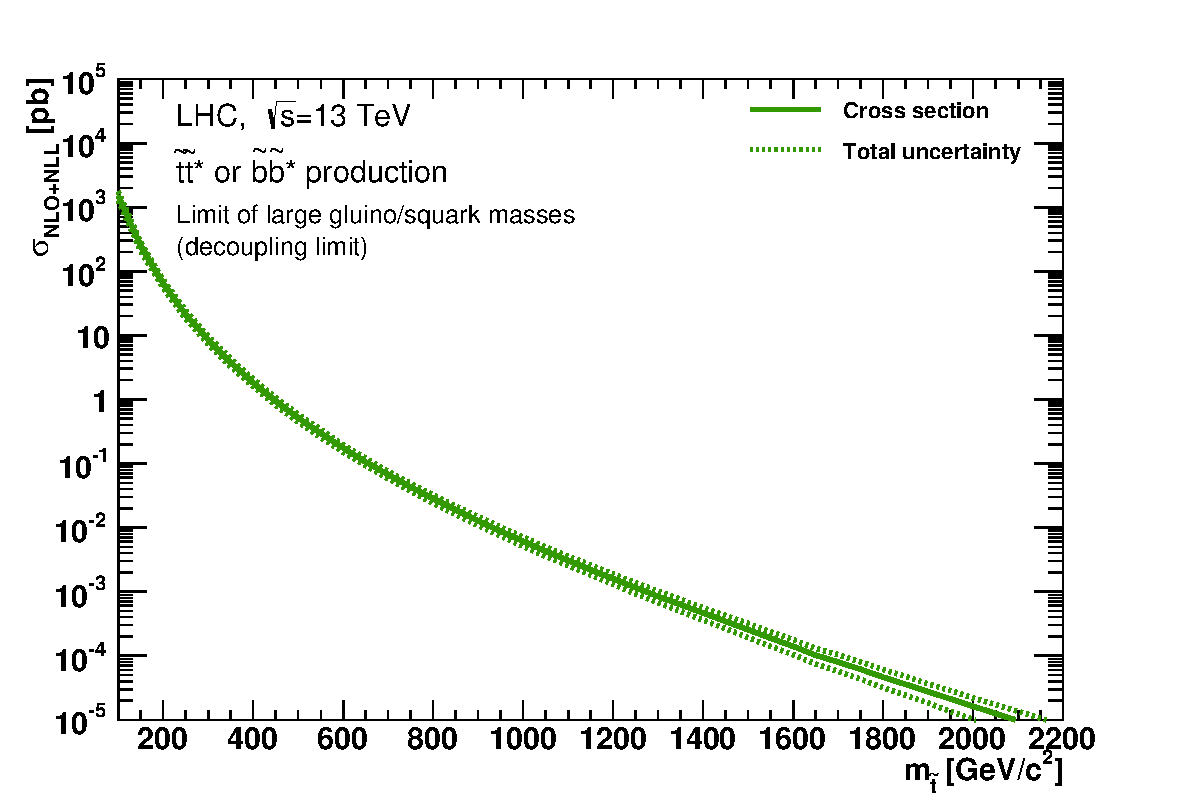
\includegraphics[width=0.3\textwidth]{figs/theory/xs_stop_100_2200.pdf}
\caption{The production cross sections of SUSY particles as a function
  of their masses computed at next-to-leading-order (NLO) with next-to-leading-logarithm (NLL)
  resummation at the LHC for 8\TeV (top) and 13\TeV (bottom)~\cite{NLONLL1,NLONLL2,NLONLL3,NLONLL4,NLONLL5,NLONLLerr,Borschensky:2014cia}.\label{fig:xsecsusy}}
\end{figure}


\section{Electroweak supersymmetric sector}
\label{sec:ewksusy}
In the MSSM, the description of electroweak symmetry breaking involves
two complex Higgs doublets, $H_\PQu = (H_\PQu^+, H_\PQu^0) $ and $H_\PQd = (H_\PQd^0, H_\PQd^-)$. The neutral
components of the Higgs doublets, $H^0_\PQu$ and $H_\PQd^0$, both get vacuum
expectation values,
\begin{align}
v_\PQu &= \langle H_\PQu^0\rangle~,& v_\PQd &= \langle H_\PQd^0\rangle~,
\end{align}
with their ratio being written as $\tan\beta = v_\PQu/v_\PQd$.

The superpartners of the neutral gauge bosons (neutral gauginos), and
the fermionic partners of the neutral Higgs bosons (neutral higgsinos),
$\psi^0 =(\PSB,\PSWz,\PSHdz,\PSHuz)$, mix to form the
\emph{neutralinos} $(\chiz_1, \chiz_2, \chiz_3, \chiz_4)$. Similarly, the superpartners of the charged gauge bosons
(charged gauginos) and the fermionic partners of the charged Higgs
bosons (charged higgsinos), $\psi^{\pm}=(\PSWp,\PSHup,\PSWm, \PSHdm)$ mix to form the charginos
$(\chip_1, \chip_2, \chim_1, \chim_2)$. In this gauge-eigenstate basis, the neutralino
and chargino mass terms in the Lagrangian are
\begin{equation}
\mathcal L_{\mathrm{MSSM}} \supset -\frac{1}{2}\psi^{0T}\mathbf{M}_N \psi^0 -\frac{1}{2}\psi^{\pm T}\mathbf{M}_C \psi^{\pm} + \mathrm{h.c.}~,
\end{equation}
with the neutralino mass matrix,
\begin{equation}
\mathbf{M}_N =\left (  \begin{matrix}
M_1 & 0 & -m_\PZ s_Wc_{\beta} & m_\PZ s_\PW s_{\beta} \\
0& M_2 & -m_\PZ c_Wc_{\beta} & -m_\PZ c_\PW s_{\beta} \\
-m_\PZ s_\PW c_{\beta}& m_\PZ c_\PW c_{\beta} & 0 & -\mu\\
m_\PZ s_\PW s_{\beta}& -m_\PZ c_\PW s_{\beta} & \mu & 0
\end{matrix}\right)~,
\end{equation}
where $s_\PW = \sin\theta_\PW$, $c_W=\cos\theta_\PW$, $\theta_W$ is the
weak mixing angle, $s_{\beta} = \sin\beta$, $c_{\beta} =
\cos\beta$, and $M_2$ and $M_1$ are the wino and bino masses, respectively.
Likewise, the chargino mass matrix is
\begin{equation}
\mathbf{M}_C =\left (  \begin{matrix}
0 & \mathbf{X}^T \\
 \mathbf{X}& 0
\end{matrix}\right), ~\mathrm{where} ~ \mathbf{X} = \left (  \begin{matrix}
M_2 & \sqrt{2}m_Ws_{\beta}\\
 \sqrt{2}m_Wc_{\beta}& \mu
\end{matrix}\right)~.
\end{equation}
The eigenvalues of these matrices are the masses of the
neutralinos and charginos.

\section{Naturalness in supersymmetry}
\label{sec:susynaturalness}

For SUSY to provide a ``natural'' solution to the gauge hierarchy problem,
the top squark, bottom squark, and gluino must have masses below a few
TeV, making them accessible at the CERN LHC. To make this statement
quantitative, we first need to define a measure of
fine-tuning, such as~\cite{Brust:2011tb,naturalSUSY}:
\begin{equation}
\Delta = \frac{\Delta(m^2_\PH)}{m^2_\PH}~.
\end{equation}
Other measures of fine-tuning are possible, such as the one given by Barbieri and Giudice~\cite{Barbieri:1987fn,Katz:2014mba}:
\begin{equation}
\Delta_x = \abs{\frac{\partial \log m^2_\PZ}{\partial \log x}}~,
\end{equation}
which quantifies the sensitivity of the $\PZ$-boson mass to
an underlying, high-energy scale parameter $x$. Although no single
measure of fine-tuning is perfect, each has its merits and can act as a proxy for our
intuitive sense of fine-tuning~\cite{Baer:2013gva}. For a model to be natural, it is traditionally desired that
$\Delta\lesssim10$, which corresponds to 10\% fine-tuning.

In the decoupling limit of the MSSM at tree-level, the mass of the
physical Higgs boson satisfies
\begin{equation}
m^2_\PH = -2(m_{\PH_\PQu}^2 + |\mu|^2) =  m_\PZ^2\cos^2(2\beta)  ~.
\end{equation}
Due to this tree-level relation between $\mu$, which controls the
masses of the higgsinos, and $m^2_\PH$, we expect both $\mu$ to be
small and the higgsinos to be light in order to keep $m^2_\PH$
small. When $\mu$ is small ($\mu \ll M_1, M_2$), the two lightest
neutralinos and the lightest chargino are higgsino-like and their
masses are close together~\cite{PhysRevD.37.2515},
\begin{align}
m_{\chiz_1} &= |\mu| + \frac{m_Z^2(1+s_{\beta})(\mu - M_1c_W^2-M_2s_W^2)}{2(\mu-M_1)(\mu-M_2)} + \cdots\\
m_{\chiz_2} &= |\mu| + \frac{m_Z^2(1-s_{\beta})(\mu + M_1c_W^2+M_2s_W^2)}{2(\mu+M_1)(\mu+M_2)} + \cdots\\
m_{\chipm_1} &= |\mu| - \frac{m_W^2(\mu + M_2\sin 2\beta)}{M_2^2-\mu^2} + \cdots~.
\end{align}
Fig.~\ref{fig:neutralinos} shows the mass differences
$m_{\chipm_1}-m_{\chiz_1}$ and $m_{\chiz_2}-m_{\chiz_1}$ as a function of the wino mass $M_2$.

\begin{figure}[tb!]
\centering
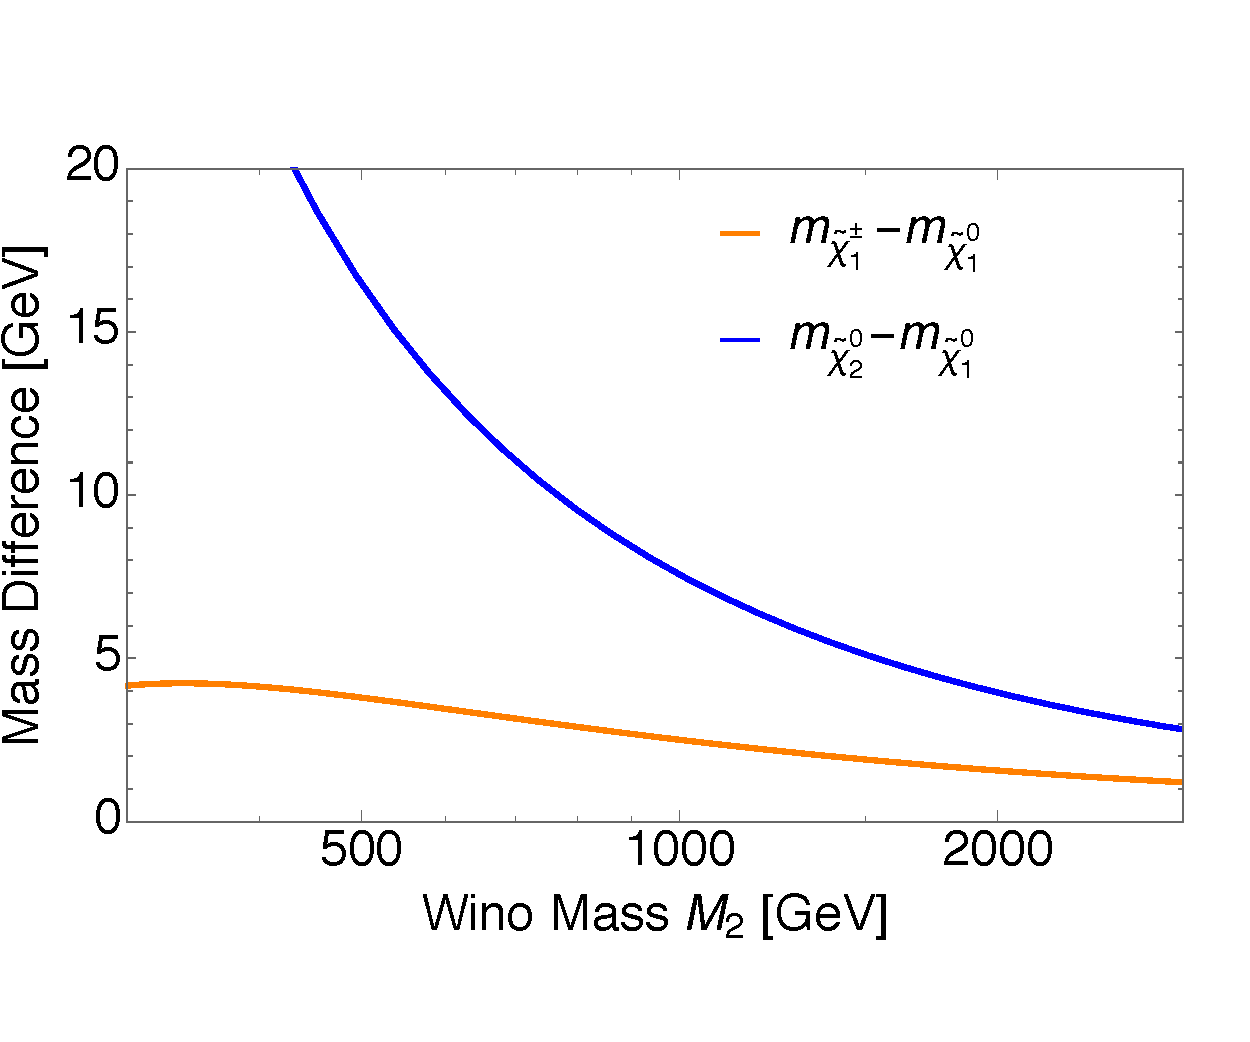
\includegraphics[width=0.8\textwidth,clip=true,viewport= 0 30 610 450]{figs/theory/neutralinos.pdf}
\caption{The mass difference between the lightest chargino and the
  lightest neutralino as a function of the wino mass $M_2$
  assuming $\tan\beta=10$, $\mu=200 \GeV$, and $M_1 = 3 \TeV$.\label{fig:neutralinos}}
\end{figure}

There are additional considerations at loop level. In particular the
top squark has a large radiative correction which partially cancels
with the contribution from the top quark in Eqn.~\ref{eqn:toploop}:
\begin{fmffile}{higgs2}
\begin{align}
\Delta(m^2_\PH) &= \quad\parbox{20mm}{\fmfreuse{fermion}} \quad + \quad
\parbox{20mm}{
\begin{fmfgraph*}(20,20)
\fmfkeep{boson}
\fmfleft{i} 
\fmfright{o} 
\fmf{dashes}{i,v}
\fmf{dashes,right,tension=0.7,label=$\PSQt_{1,,2}$}{v,v}
\fmf{dashes}{v,o}
\fmfv{label=$\PH$,label.angle=90}{i}
\end{fmfgraph*}}
 \quad + \quad
\parbox{20mm}{
\begin{fmfgraph*}(20,20)
\fmfkeep{sunset}
\fmfleft{i}
\fmfright{o}
\fmf{dashes}{i,v1}
\fmf{dashes}{v2,o}
\fmf{dashes,left,tension=.3,label=$\PSQt_{1,,2}$}{v1,v2}
\fmf{dashes,left,tension=.3}{v2,v1}
\fmfv{label=$\PH$,label.angle=90}{i}
\end{fmfgraph*}} \quad + \quad\cdots\\
 &= -\frac{3|y_\PQt|^2}{8\pi^2}\Lambda_{\mathrm{UV}}^2 +
  \sum_{i=1}^{2} \left ( \frac{3|y_\PQt|^2}{16\pi^2}\Lambda_{\mathrm{UV}}^2 - \frac{3|y_\PQt|^2m_{\PSQt_i}^2}{8\pi^2}\log\left (\frac{\Lambda_{\mathrm{UV}}}{m_{\PSQt_i}}\right ) \right )+ \cdots \\
 &= -\sum_{i=1}^{2} \left ( \frac{3|y_\PQt|^2m_{\PSQt_i}^2}{8\pi^2}\log\left (\frac{\Lambda_{\mathrm{UV}}}{m_{\PSQt_i}}\right ) \right )+ \cdots~.
\label{eqn:stoploop}
\end{align}
\end{fmffile}
The cancellation of the term proportional to $\Lambda_{\mathrm{UV}}^2$
in Eqn.~\ref{eqn:stoploop} is one of the major successes of SUSY as a candidate for physics beyond
the SM. The sensitivity of the Higgs mass to ultraviolet new
physics is now logarithmic instead of quadratic. If SUSY were an exact
symmetry (and $m_\PQt=m_{\PSQt_{1,2}}$) then the cancellation would be
exact and there would be no further hierarchy problem. As it stands, however, we know SUSY is broken, and the
remaining term may also be large depending on the difference in masses
between the top quark and top squarks. Therefore, naturalness places constraints on the allowed masses of the top
squarks given an ``acceptable'' level of fine tuning.

Very roughly, naturalness requires $m_{\PSQt_{i}}\lesssim
400 \GeV$ if $\Lambda_{\mathrm{UV}}\approx
10\TeV$, implying a fine tuning of the order of
10\%~\cite{Brust:2011tb,Craig:2013cxa}. 
%A more complete treatment takes into
%account top squark mixing~\cite{Kitano:2006gv,naturalSUSY},
%\begin{equation}
%\Delta(m^2_\PH) = \frac{3|y_\PQt|^2}{4\pi^2}\left ( m_{Q_3}^2 + m_{U_3}^2 + |A_t|^2 \right ) \log\left(
 % \frac{\Lambda_{\mathrm{mess}}}{m_{\PSQt}} \right)
%\end{equation}

There is also a two-loop contribution to the Higgs mass parameter from
the gluino, which is closely related to the one-loop contribution to
the top squark mass from the gluino~\cite{Craig:2013cxa}:
\begin{fmffile}{higgs3}
\begin{align}
\Delta (m^2_{\PSQt_{i}}) & = \quad \parbox{20mm}{
\begin{fmfgraph*}(20,20)\fmfkeep{gluinosunset}
\fmfleft{i}\fmfright{o}
\fmf{dashes}{i,v1}
\fmf{dashes}{v2,o}
\fmf{gluon,left,tension=.3,label=$\sGlu$}{v1,v2}
\fmf{plain,left,tension=.3,label=$\PQt$}{v2,v1}
\fmfv{label=$\PSQt_{i}$,label.angle=90}{i}
\fmffreeze\fmf{plain,left,tension=.3}{v1,v2}
\end{fmfgraph*}} + \quad \cdots\\
&= \frac{2g^2_{\mathrm{s}}m_{\sGlu}^2}{3\pi^2}\log\left(\frac{\Lambda_{\mathrm{UV}}}{m_{\sGlu}}\right) + \cdots~,
\label{eqn:gluinoloop}
\end{align}
\end{fmffile}
With this, we have roughly that $m_{\sGlu} \lesssim 2 m_{\PSQt_{i}}$.

Prior to the work described in this thesis, constraints from collider
searches, especially those from the LHC at
$\sqrt{s}=7\TeV$~\cite{Chatrchyan:2012pka,razor2010,razorPRL,Chatrchyan:2012jx,Chatrchyan:2012sa,Aad:2012ywa,Aad:2012xqa,Aad:2012tx,Aad:2012yr,Aad:2012naa,Aad:2012fqa,Aad:2012pq,Aad:2012pxa,Aad:2012hba},
pushed the allowed mass range for neutralinos and charginos up to
$\gtrsim200\GeV$, for top and bottom squarks up to $\gtrsim500
\GeV$, and for gluinos up to $\gtrsim1 \TeV$. Taking into consideration the
experimental and theoretical constraints at tree, one-loop, and
two-loop levels, there are three requirements for a minimal natural
SUSY spectrum~\cite{naturalSUSY}:
\begin{enumerate}[(a)]
\item quasi-degenerate higgsino-like chargino $\chipm_1$ and two
  neutralinos $\chiz_1, \chiz_2$, below
  $200 - 350 \GeV$, 
\item two top squarks $\sTop_{1,2}$ and one (left-handed) $\sBot_1$ below
  $500-700 \GeV$, and
\item a gluino below $1 - 1.5 \TeV$.
\end{enumerate}

\section{Soft supersymmetry breaking}
\label{sec:softsusybreaking}

Since superpartners have not already been discovered with exactly
the same masses as the SM particles, we know SUSY is a broken
symmetry. However, the form of nature of SUSY breaking is constrained
by the fact that we should preserve the relationships between the
dimensionless couplings that create the cancellation of the quadratic
divergence of the Higgs mass. This means that the effective Lagrangian
of the MSSM can be written as the sum of two terms,
\begin{equation}
\mathcal L_\mathrm{MSSM}+\mathcal L_\mathrm{MSSM}^\mathrm{soft}~,
\end{equation}
where $\mathcal L_\mathrm{MSSM}$ contains all of the gauge and Yukawa
interactions that preserve SUSY, and $\mathcal
L_\mathrm{MSSM}^\mathrm{soft}$ violates SUSY but contains only mass
terms and couplings with \emph{positive} mass dimension. Explicitly, the
soft SUSY breaking part of the MSSM Lagrangian can be written~\cite{susyprimer},
\begin{align}
\mathcal
  L_\mathrm{MSSM}^\mathrm{soft}&=-\frac{1}{2}\left(M_3\widetilde{g}\widetilde{g}
                                 + M_2\widetilde W\widetilde W +
                                 M_1\widetilde B\widetilde B +
                                 \mathrm{h.c.}\right)\\
&-\left(\widetilde{U}^\mathrm{c}\boldsymbol{a_\PQu}\widetilde{Q} H_\PQu -
  \widetilde{D}^\mathrm{c} \boldsymbol{a_\PQd}\widetilde Q H_\PQd -
  \widetilde{E}^\mathrm{c} \boldsymbol{a_\Pe} \widetilde L H_\PQd +
  \mathrm{h.c.}\right)\\
&-\widetilde Q^{\dagger} \boldsymbol{m_{\widetilde{\mathrm{Q}}}^2}\widetilde Q - \widetilde
  L^{\dagger}\boldsymbol{m_{\widetilde{\mathrm{L}}}^2} \widetilde L
-\widetilde U^\mathrm{c}\boldsymbol{m_{\widetilde{\mathrm{U}}^\mathrm{c}}^2} \widetilde
  U^{\mathrm{c}\dagger} - \widetilde D^\mathrm{c}\boldsymbol{m_{\widetilde{\mathrm{D}}^\mathrm{c}}^2} \widetilde
  D^{\mathrm{c}\dagger} - \widetilde{E}^\mathrm{c}\boldsymbol{m_{\widetilde{\mathrm{E}}^\mathrm{c}}^2} \widetilde
  E^{\mathrm{c}\dagger} \\
&-m_{\PH_\PQu}^2H^{\ast}_\PQu H_\PQu - m_{\PH_\PQd}^2H^{\ast}_\PQd H_\PQd -
  (bH_\PQu H_\PQd + \mathrm{h.c.})~,
\end{align}
where $M_3$, $M_2$, and $M_1$ are the gluino, wino, and bino mass
terms, respectively. Each of $\boldsymbol{a_\PQu} $, $\boldsymbol{a_\PQd}$, $\boldsymbol{a_\Pe}$ is a complex $3\times3$ matrix in generation space,
with dimensions of mass. They are in one-to-one correspondence with the Yukawa couplings of the
superpotential. Each of $\boldsymbol{m_{\widetilde{\mathrm{Q}}}^2}$, $\boldsymbol{m_{\widetilde{\mathrm{L}}}^2}$,
$\boldsymbol{m_{\widetilde{\mathrm{U}}^\mathrm{c}}^2}$, $\boldsymbol{m_{\widetilde{\mathrm{D}}^\mathrm{c}}^2}$,
$\boldsymbol{m_{\widetilde{\mathrm{E}}^\mathrm{c}}^2}$ is a $3\times3$  matrix in
generation space that can have complex entries, but must be hermitian
so that the Lagrangian is real. Finally, $m_{\PH_\PQu}^2$ and $m_{\PH_\PQd}^2$
are squared-mass terms and $b$ is a cross term in the Higgs potential.

If the largest mass scale associated with the soft SUSY breaking terms is $m_\mathrm{soft}$, then the additional non-supersymmetric corrections to the Higgs
mass squared must vanish in the $m_\mathrm{soft}\to0$ limit, so by dimensional analysis they cannot be proportional to
$\Lambda_{\mathrm{UV}}^2$. They also cannot be proportional to
$m_{\mathrm{soft}}\Lambda_{\mathrm{UV}}$ because momentum loop
integrals do not depend linearly on the cut-off scale. Thus they must be
proportional to $m_\mathrm{soft}^2$. Following a similar line of
argument, we expect that the coefficients of the soft SUSY
breaking terms are also proportional to appropriate powers of $m_\mathrm{soft}$:
\begin{align}
M_1,M_2,M_3,\boldsymbol{a_\PQu},\boldsymbol{a_\PQd},\boldsymbol{a_\Pe} &\sim m_\mathrm{soft}~,\\
\boldsymbol{m_{\widetilde{\mathrm{Q}}}^2}, \boldsymbol{m_{\widetilde{\mathrm{L}}}^2},
                                                                 \boldsymbol{m_{\widetilde{\mathrm{U}}^\mathrm{c}}^2},
                                                                 \boldsymbol{m_{\widetilde{\mathrm{D}}^\mathrm{c}}^2},
                                                                 \boldsymbol{m_{\widetilde{\mathrm{E}}^\mathrm{c}}^2},
                                                                 m_{\PH_\PQu}^2,
                                                                 m_{\PH_\PQd}^2,
  b&\sim m_\mathrm{soft}^2~.
\end{align}



\section{Renormalization group in supersymmetry}
\label{sec:rgemssm}
The one-loop beta functions in the MSSM are modified with respect to
the ones in the SM due to the additional particle
content. Numerically, they become,
\begin{align}
\frac{\rd g_1}{\rd\log\mu} &=\frac{g_1^3}{20\pi^2} \left( \frac{33}{4} \right)~,\\
\frac{\rd g_2}{\rd\log\mu} &= \frac{g_2^3}{16\pi^2}\left( 1 \right)~,\\
\frac{\rd g_3}{\rd\log\mu} &= \frac{g_3^3}{16\pi^2}\left( -3\right)~.
\end{align}
Fig.~\ref{fig:unification}, shows how the gauge couplings, expressed
as $\alpha^{-1}_{i} = 4\pi/g_i^2$, run in both the SM and the MSSM~\cite{susyprimer}. Unlike the SM, the MSSM includes the right
particle content to ensure that the gauge couplings can unify at a
mass scale $\sim2 \times10^{16} \GeV$~\cite{susyprimer}.

\begin{figure}
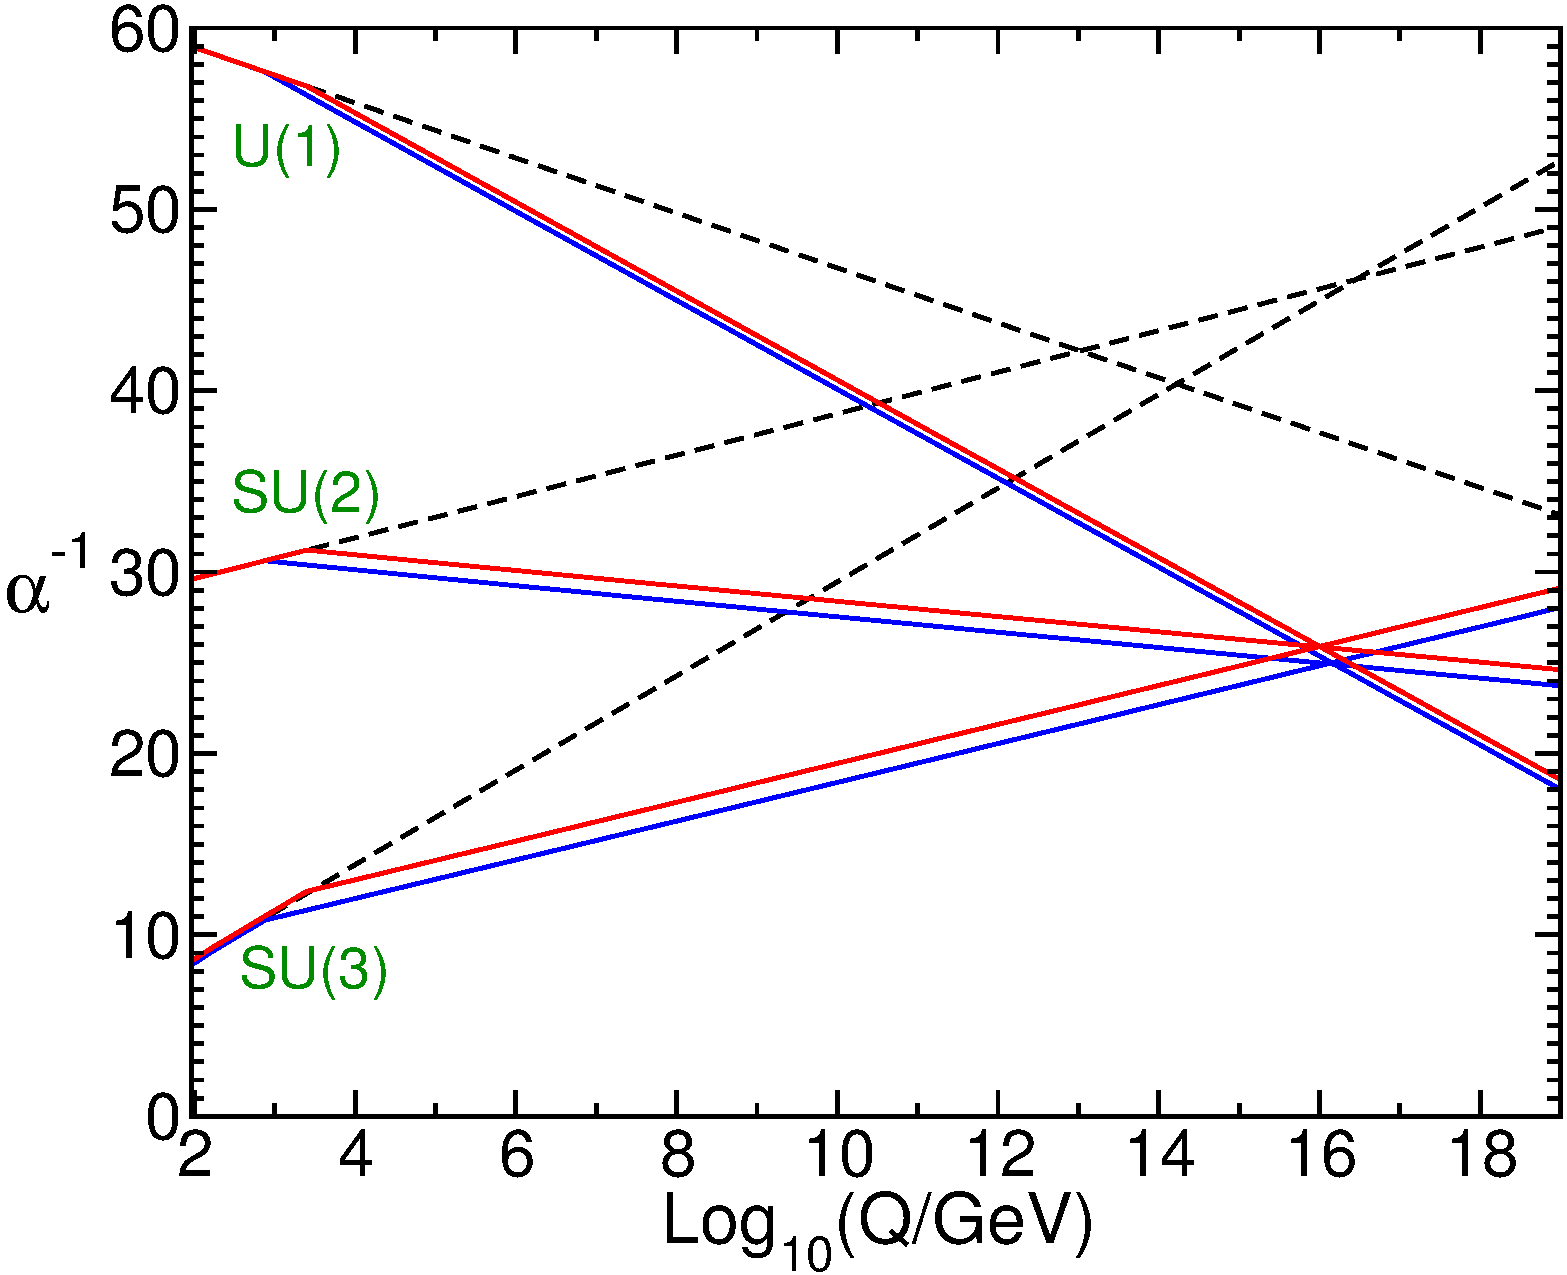
\includegraphics[width=0.49\textwidth]{figs/theory/unification.pdf}
\caption{Two-loop renormalization group evolution of the inverse
gauge couplings $\alpha^{-1}_i(\mu)$ in the SM (dashed lines) and the
MSSM (solid lines). In the MSSM case, the sparticle masses are treated
as a common threshold varied between $500\GeV$ and $1.5\TeV$, and
$\alpha_3(m_\PZ)$ is varied between $0.117$ and
$0.121$.~\cite{susyprimer}.\label{fig:unifcation}}
\end{figure}

\section{Simplified natural supersymmetry models}
\label{sec:sms}

\begin{figure}[htb!]
\centering
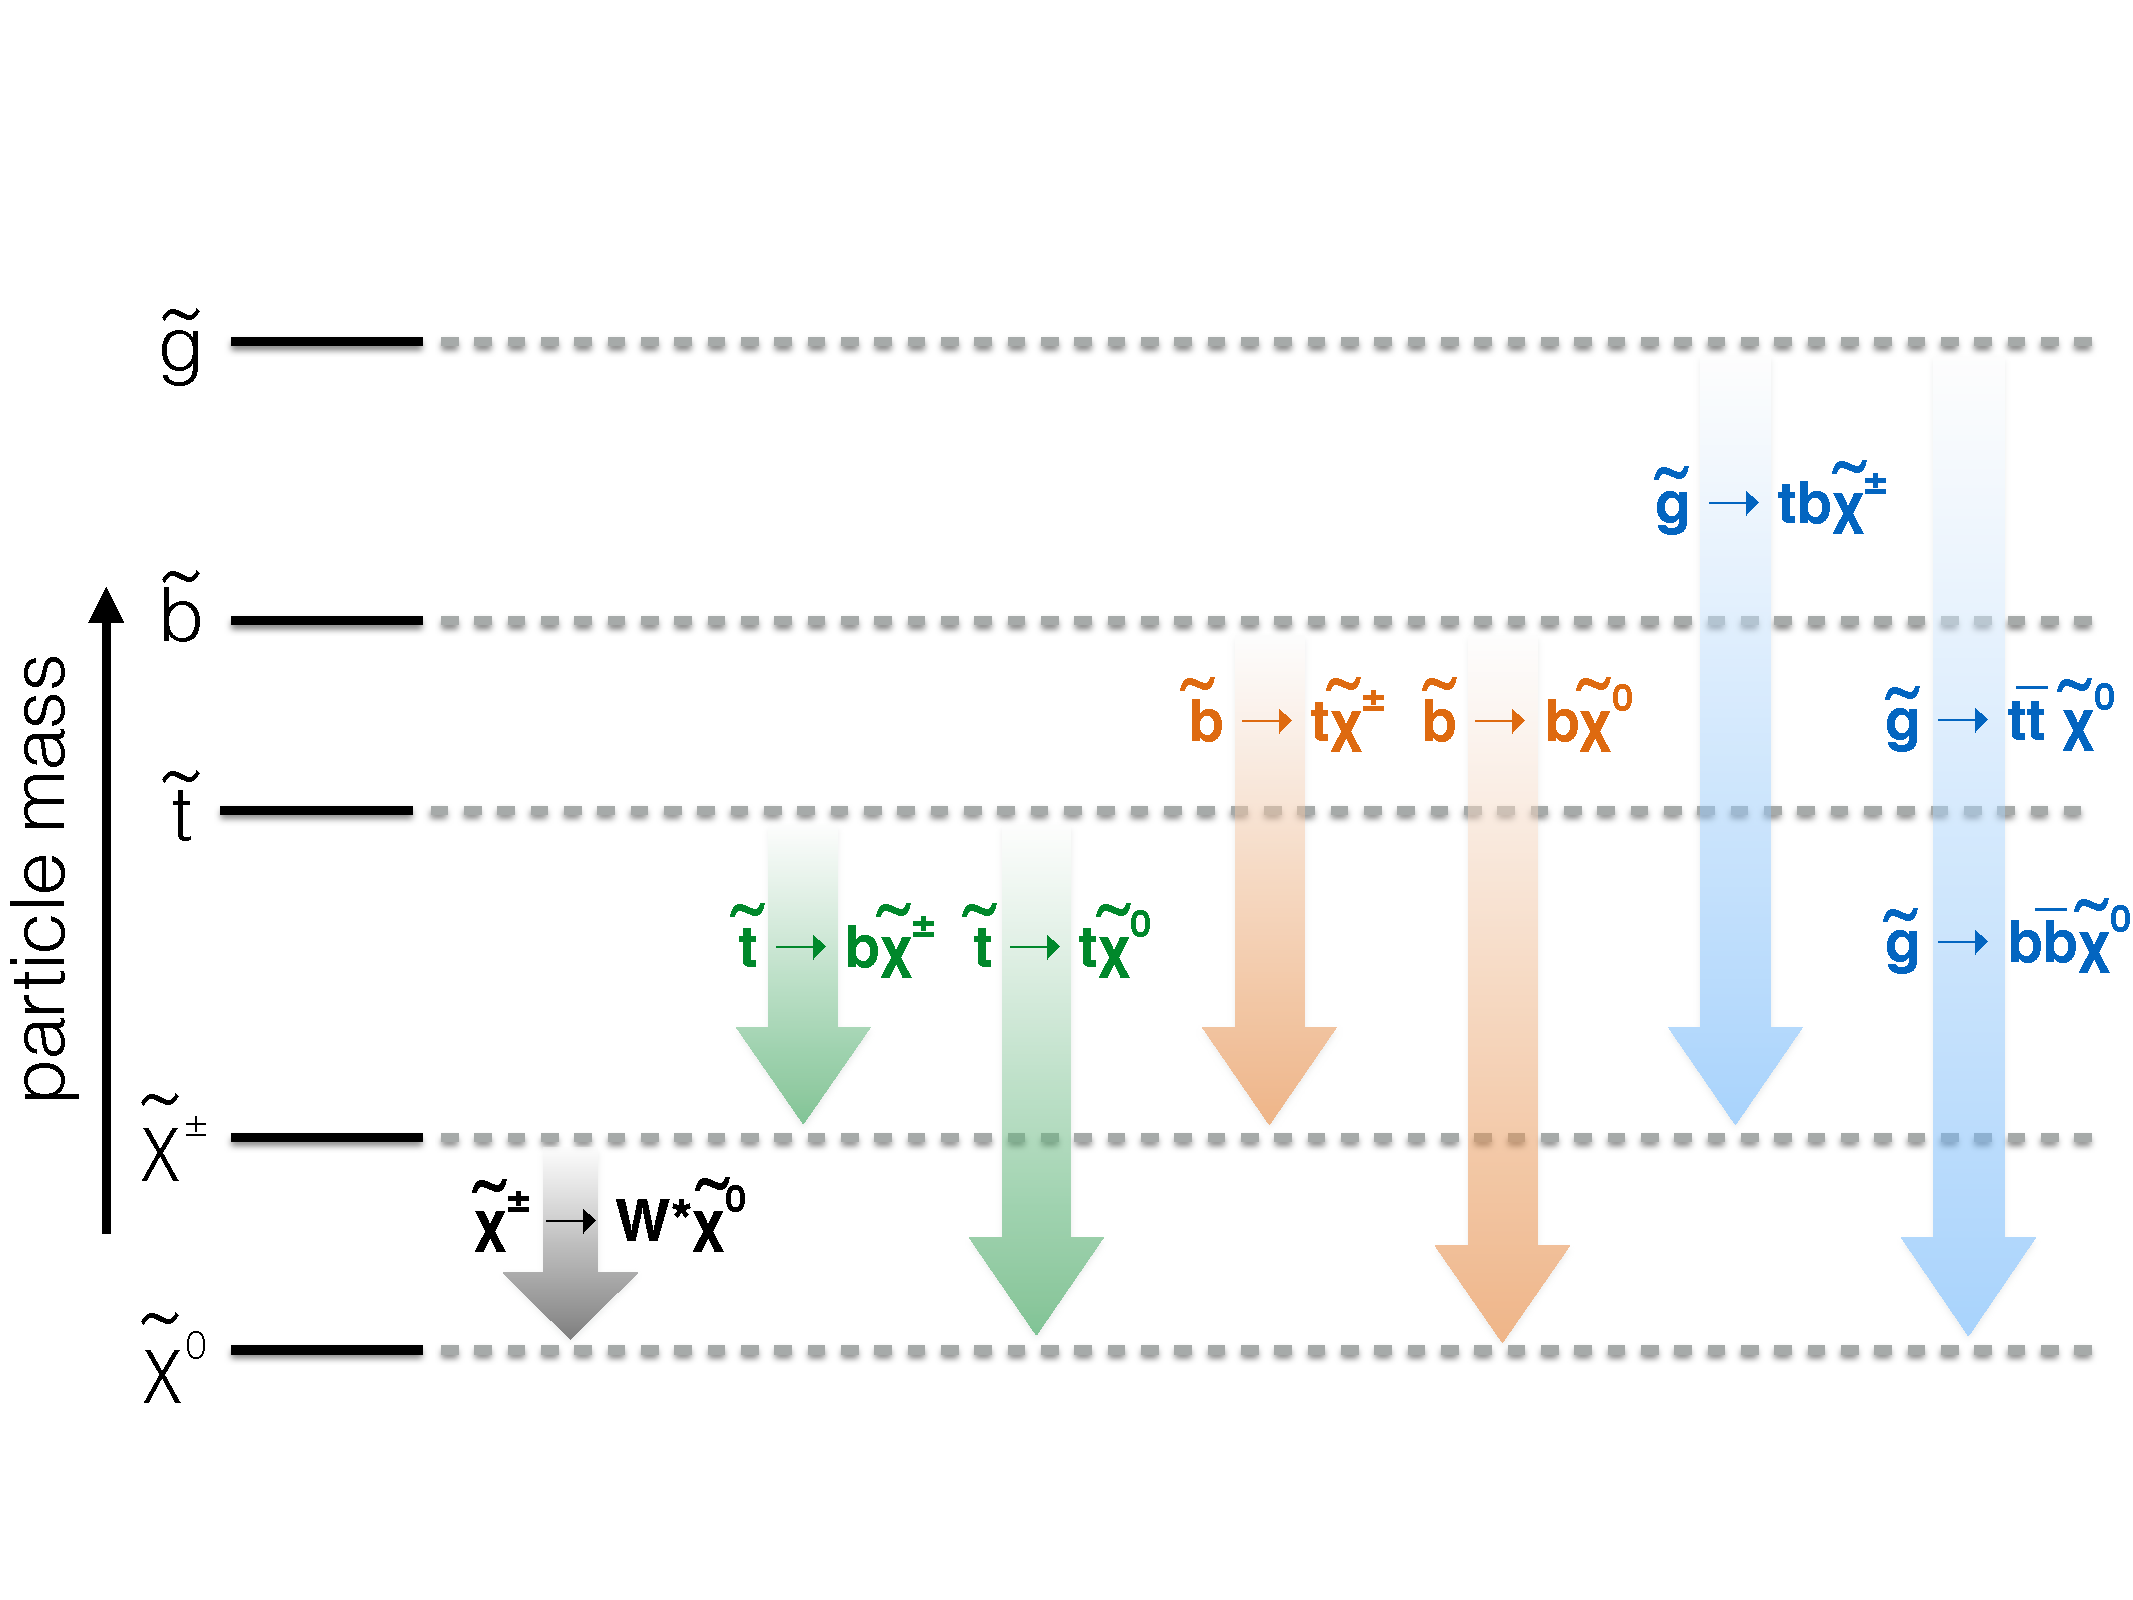
\includegraphics[width=0.85\textwidth]{figs/analysis8TeV/naturalSpectrum.pdf}
\caption{\label{fig:spectrum} The simplified natural SUSY spectrum
  considered in this thesis, along with the assumed decay modes~\cite{razor8TeV,jmgd}.}
\end{figure}

Motivated by the discussion of Sec.~\ref{sec:susynaturalness}, we may
outline an explicit minimal natural SUSY scenario. In this scenario, the LSP is the lightest neutralino $\chiz_1$ while the NLSP
is the lightest chargino $\chipm_1$. They are both higgsinos and
quasi-degenerate. To reduce the dimensionality of this parameter
space, and the NLSP-LSP mass splitting is taken to be 5\GeV.
This specific choice of mass splitting is supported by Fig.~\ref{fig:neutralinos}, but does not
have a large impact on the results of the interpretation. 
The NLSP decays to the LSP and a virtual $\PW$ boson ($\chipm_1 \to
\PW^{\ast} \chiz_1$), whose decay products mostly have too low
momentum to identified. The other SUSY particles accessible at the LHC are the gluino and the
lightest top and bottom squarks. All other SUSY particles are
assumed to be too heavy to participate in the interactions. We only allow
the gluino decay modes involving third-generation quarks because their
corresponding decay rates are enhanced if the masses of the third-generation squarks are lighter
than those of the first two generations. The SUSY particles and their possible decay modes within this natural SUSY
spectrum are summarized in Fig.~\ref{fig:spectrum}.

In the context of this natural spectrum, several simplified
models~\cite{ArkaniHamed:2007fw,Alwall:2008ag,Alwall:2008va,Alves:2011sq,Alves:2011wf,Graesser:2012qy}
are considered in Ch.~\ref{ch:analysis8TeV} and
Ch.~\ref{ch:analysis13TeV} for gluino pair production based on three-body gluino
decays, in which each gluino decays to one of the following final states~\cite{SUS-11-016}:
\begin{itemize}
\item a top quark (antiquark) and a bottom antiquark (quark),
  and the NLSP; 
\item a top quark-antiquark ($\ttbar$) pair and the LSP;
\item a bottom quark-antiquark ($\bbbar$) pair and the LSP.
\end{itemize}
The full range of branching fractions to the three possible decay modes ($\bbbar\chiz_{1}$,
$\cPqb\cPaqt\chip_1$ or $\cPaqb\cPqt\chim_1$, and $\ttbar\chiz_{1}$) is considered. 
Furthermore, we separately consider the case in which each gluino
decays to
\begin{itemize}
\item a first or second generation quark-antiquark ($\qqbar$) pair and the LSP.
\end{itemize}

In addition, several simplified models are considered for
the production of top-squark pairs, in which each top squark decays to
one of the following final state:
 \begin{itemize}
\item a bottom quark and the NLSP;
\item a top quark and the LSP.
\end{itemize}
Similarly, the full range of branching fractions to the both possible
decay modes ($\cPqb\chip_1$ or $\cPaqb\chim_1$, and $\cPqt\chiz_1$) is considered.

The corresponding Feynman diagrams showing the event topologies are displayed in
Fig.~\ref{fig:SMSDiagrams}.

\begin{figure*}[thb!]
\centering
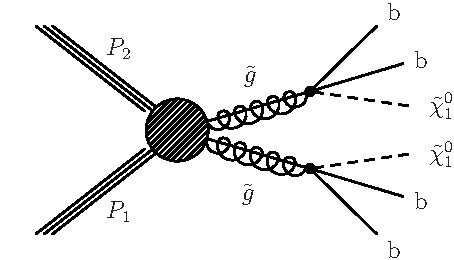
\includegraphics[width=0.45\textwidth]{figs/theory/T1bbbb.pdf}
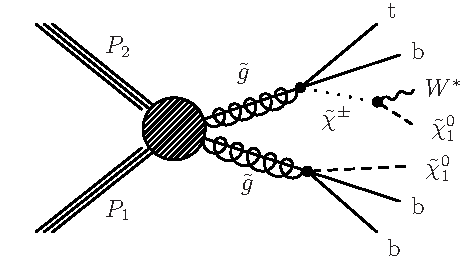
\includegraphics[width=0.45\textwidth]{figs/theory/T1tbbb.pdf}\\
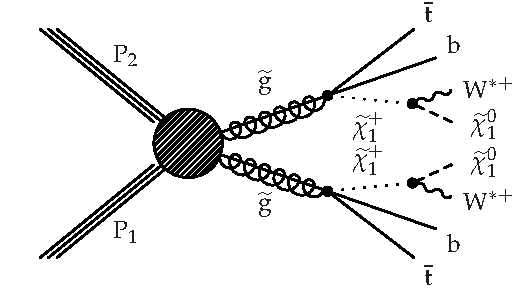
\includegraphics[width=0.45\textwidth]{figs/theory/T1ttbb.pdf} 
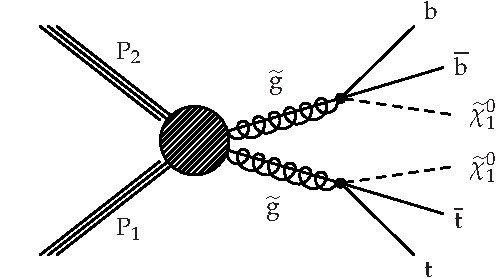
\includegraphics[width=0.45\textwidth]{figs/theory/T1tbtb.pdf} \\
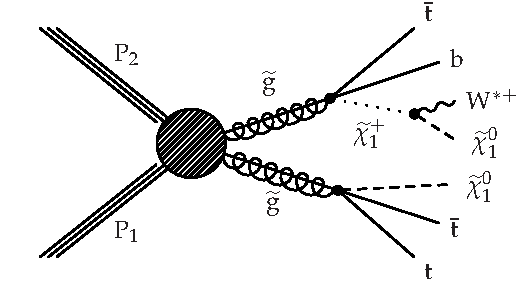
\includegraphics[width=0.45\textwidth]{figs/theory/T1tttb.pdf}
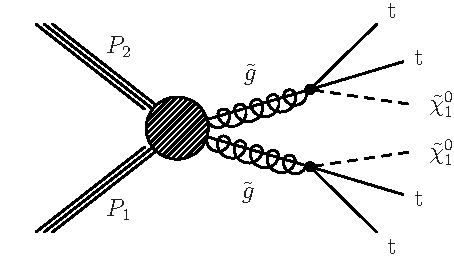
\includegraphics[width=0.45\textwidth]{figs/theory/T1tttt.pdf} \\
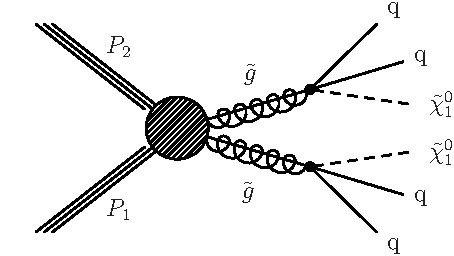
\includegraphics[width=0.45\textwidth]{figs/theory/T1qqqq.pdf} 
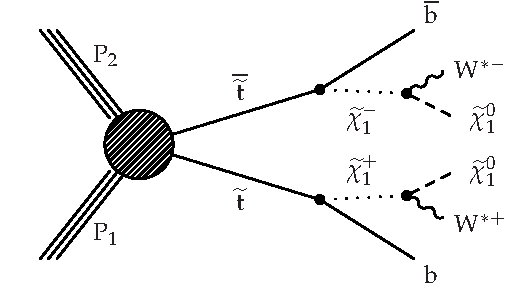
\includegraphics[width=0.45\textwidth]{figs/theory/T2bw.pdf} \\
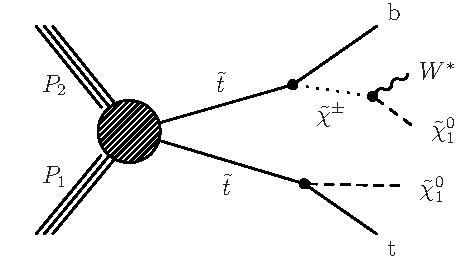
\includegraphics[width=0.45\textwidth]{figs/theory/T2tb.pdf}
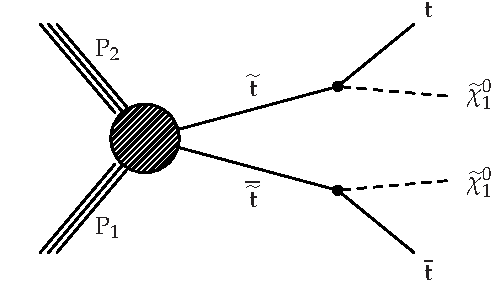
\includegraphics[width=0.45\textwidth]{figs/theory/T2tt.pdf}
\caption{Diagrams displaying the event topologies of gluino and top-squark pair production
  considered in this thesis~\cite{razor8TeV,jmgd}.\label{fig:SMSDiagrams}}
\end{figure*}

\subsection{Technical implementation of chargino decays in \PYTHIA}
To simplify the treatment of the sparticle decays in \PYTHIA v6.4.26, we directly implement three-body decays of
the form $\chipm_1 \to \chiz_1 \mathrm{f} \mathrm{f}^{\prime}$, with branching ratios
as shown in Tab.~\ref{tab:nlspbr}.
\begin{table}
\centering
\begin{tabular}{l|r}
\hline\hline
decay mode & branching ratio \\\hline
$\chip_1 \to \chiz_1 \cPqu \cPaqd$ &  35\%\\
$\chip_1 \to \chiz_1 \cPqc \cPaqs$ &  35\%\\
$\chip_1 \to \chiz_1 \Pep \PGne$ &  12\%\\
$\chip_1 \to \chiz_1 \PGmp \PGnGm$ &  12\%\\
$\chip_1 \to \chiz_1 \PGtp \PGnGt$ &  6\%\\
\hline\hline
\end{tabular}
\caption{\label{tab:nlspbr}Table of branching ratios implemented in
  \PYTHIA v6.4.26 for the NLSP
  $\chipm_1$ in the simplified natural SUSY model considered in this chapter.}
\end{table}